% SPDX-FileCopyrightText: 2023 SAP SE
%
% SPDX-License-Identifier: Apache-2.0
%
% This file is part of FEDEM - https://openfedem.org

%%%%%%%%%%%%%%%%%%%%%%%%%%%%%%%%%%%%%%%%%%%%%%%%%%%%%%%%%%%%%%%%%%%%%%%%%%%%%%%%
%
% FEDEM User Guide.
%
%%%%%%%%%%%%%%%%%%%%%%%%%%%%%%%%%%%%%%%%%%%%%%%%%%%%%%%%%%%%%%%%%%%%%%%%%%%%%%%%

\Chapter{Mechanism Analysis}{mechanism-analysis}

Now that you can assemble a model and implement a control system,
you are ready to analyze the mechanism.
This chapter describes methods of mechanism analysis in Fedem, including
descriptions of setting up, starting, processing, and stopping the analyses.

Sections in this chapter address the following topics:

\begin{itemize}
\item
  \protect\hyperlink{overview-of-fedem-analyses}
                    {Overview of Fedem analyses}
\item
  \protect\hyperlink{solver-tools}
                    {Solver tools}
\item
  \protect\hyperlink{model-reduction}
                    {Model reduction}
\item
  \protect\hyperlink{model-reduction-in-nastran}
                    {Model reduction in Nastran}
\item
  \protect\hyperlink{dynamics-analysis}
                    {Dynamics analysis}
\item
  \protect\hyperlink{stress-recovery-analysis}
                    {Stress recovery analysis}
\item
  \protect\hyperlink{mode-shape-recovery-analysis}
                    {Mode shape recovery analysis}
\item
  \protect\hyperlink{strain-rosette-analysis-1}
                    {Strain rosette analysis}
\item
  \protect\hyperlink{strain-coat-analysis-1}
                    {Strain coat analysis}
\item
  \protect\hyperlink{direct-linear-analysis-of-fe-parts}
                    {Direct linear analysis of FE Parts}
\item
  \protect\hyperlink{interaction-during-processing}
                    {Interaction during processing}
\item
  \protect\hyperlink{deleting-results}
                    {Deleting results}
\item
  \protect\hyperlink{automated-curve-export-from-multiple-result-database-files}
                    {Automated curve export from multiple result database files}
\item
  \protect\hyperlink{batch-execution-of-solver-processes}
                    {Batch execution of solver processes}
\item
  \protect\hyperlink{how-to-read-error-messages-from-the-solvers}
                    {How to read error messages from the solvers}
\item
  \protect\hyperlink{using-simulation-events}
                    {Using simulation events}
\end{itemize}

\clearpage


%%%%%%%%%%%%%%%%%%%%%%%%%%%%%%%%%%%%%%%%%%%%%%%%%%%%%%%%%%%%%%%%%%%%%%%%%%%%%%%%
\Section{Overview of Fedem analyses}{overview-of-fedem-analyses}

\subsection{Model reduction}

To speed up the dynamics simulation and other mechanism analyses,
Fedem first performs the model reduction process.
During model reduction, individual parts (FE models) in the mechanism assembly
are reduced to superelements with external nodes at those points which connect
parts and other mechanism elements.

Fedem uses a Component Mode Synthesis (CMS) model reduction method that replaces
the internal nodal DOFs with a set of static and component modes.
The model reduction process for each part generates superelement mass- and
stiffness matrices, which are then assembled into the system mass and stiffness
matrices in the dynamics simulation.
See the \FedemTGuide{Chapter 3, "Model Reduction"}
for more information about the Fedem model reduction process.

You can initiate the model reduction process manually at any time
(see \refSection{model-reduction}{Model reduction}).
Alternatively, you may also perform the model reduction in Nastran
(see \refSection{model-reduction-in-nastran}{Model reduction in Nastran}).


\SubSection{Dynamics analysis}{dynamics-analysis-overview}

The dynamics analysis provides the time-history solution for all displacements,
velocities, accelerations, control system variables, and derived secondary
quantities (such as internal reaction forces) in the mechanical system that are
driven by external forces and/or prescribed displacements, velocities and
accelerations.

To achieve second-order accuracy, the dynamic solution to the full system of
equations is found using Newmark time-integration and Newton-Raphson equilibrium
iterations at each time step.
For the control system, an implicit second-order Runge-Kutta method
(Lobatto IIIC) is used with Backward Euler for local error estimation.
The latter is an implicit first-order method.
See the \FedemTGuide{Chapter 7, "Dynamics Simulation"}
and {\sl Chapter 8, "Control System"}, respectively, for more information about
the dynamics analysis of the mechanical system, and the control system analysis.

See \refSection{dynamics-analysis}{Dynamics analysis}
to set up and perform the dynamics analysis.

\SubSubSection{Static equilibrium analysis}{static-equilibrium-analysis}

Before performing the dynamics simulation, Fedem may calculate an initial static
equilibrium state for the mechanism model. The static equilibrium analysis
establishes a starting point for the dynamics analysis, and eliminates the
initial system transients such as the sudden effect of applying gravity or other
external loads. In the dynamics analysis, such unbalanced forces in the initial
configuration can generate undesirable effects such as vibration of
the mechanism during the first time steps.
See the \FedemTGuide{Section 7.8, "Quasistatic equilibrium"}
for more information about the initial static equilibrium analysis.

The static equilibrium analysis determines a state for the system in which all
internal and external forces are in balance in the absence of any system motions
or inertial forces.
All system velocities and accelerations are set to zero during this analysis.

To set up the static equilibrium analysis, see
\refSubSection{initial-equilibrium-tab}{Initial Equilibrium tab}
              {dynamics-solver-advanced-mode}.

\subsubsection{Dynamic Initial Conditions}

When using the static equilibrium analysis described above,
the subsequent dynamics simulation will start from a resting position with
zero velocities and accelerations in all DOFs. In some cases, however,
it is more relevant to start the dynamics simulation from a known velocity
state in the triads and joins instead. This is possible by specifying
the {\sl Initial velocity} directly on each DOF through the respective
Property Editor panels, see \refSection{triad-properties}{Triad properties}
and \refSection{joint-properties}{Joint properties}.
This will override the global initial velocity defined in the Model Preferences
dialog box, see \refSection{model-preferences}{Model preferences}.

\Tip{If the initial condition is characterized by a uniform velocity throughout
  the model, except for a few triads or joints where the velocity is different,
  it is practical to specify the "background" velocity in the Model Preferences
  dialog box, and use the Property Editor panel only for those Triads/Joints
  having a different initial velocity.}

\Caution{Initial velocities should be used with care such that the velocity
  state specified this way is consistent throughout the model.
  If that is not the case, fictitious transients may occur
  in the first time steps of the analysis.}

When using initial conditions, it is recommended to specify velocities
for the joint DOFs also. The initial velocities at the slave triad of
the joint will then be computed automatically from the constraint
equations of the joint. However, it is possible to instead specify the
initial velocity in the slave triad (and leave the joint DOF initial
velocities to zero), if the joint DOF velocity is not known.
Fedem will then derive the corresponding
joint velocities by inverting the constraint equation of the joint.

Sometimes during the creation of a complex model, it is useful to test
the dynamics when all initial conditions are off (equal to zero).
To facilitate this without having to manually remove all the defined
initial conditions in the model file, the solver option {\tt-ignoreIC}
may be specified instead (in the Additional Solver Options dialog box,
{\sl Dynamics Solver} field,
see \refSection{additional-solver-options}{Additional solver options}).
All defined initial conditions will then be ignored (assumed zero).

If you do a static equilibrium analysis prior to the dynamics simulation, any
initial conditions specified will not affect the static equilibrium analysis
itself. However, the subsequent dynamics simulation will then start from
a configuration that is in static equilibrium,
but with a given non-zero velocity state.

\SubSubSection{Modal analysis}{modal-analysis}

The dynamics analysis gives you the option of calculating the eigenmodes
at different mechanism positions during the simulation.
These eigenmode solutions can then be used to expand the model's mode shapes
for later use in animations.
See the \FedemTGuide{Section 9.6, "Eigenvalue results"}
for more information about the modal analysis.

To specify the parameters for modal analysis, see
\refSubSection{eigenmode-tab}{Eigenmode tab}{dynamics-solver-advanced-mode}.


\SubSection{Stress recovery}{stress-recovery-1}

After performing the dynamics analysis,
a stress analysis can be conducted on the mechanism.
The stresses, strains and elastic displacements can then be calculated at
different time steps and/or mechanism positions of the dynamics analysis.
See the \FedemTGuide{Section 9.4, "Finite element stress analysis"}
for more information about the stress analysis.
See \refSection{stress-recovery-analysis}{Stress recovery analysis}
to setup and perform the stress analysis.

\clearpage


\subsection{Mode shape recovery}

A mode shape recovery analysis enables you to expand the system mode shapes
calculated during the dynamics simulation.
These mode shapes can later be animated.
See \refSection{mode-shape-recovery-analysis}{Mode shape recovery analysis}
to setup and perform the mode shape analysis.


\subsection{Strain rosette recovery}

Fedem enables you to recover strains and stresses from virtual strain gages
which are defined in a separate file.
The results are similar to those from real strain gages.
See the \FedemTGuide{Section 9.5, "Virtual strain gauges"}
for more information about the strain rosette analysis.
See \refSection{strain-rosette-analysis-1}{Strain rosette analysis}
to setup and perform the strain rosette analysis.


\subsection{Strain coat recovery}

The strain coat recovery process calculates the stresses and strains
on the strain coat elements in the model,
in a similar manner as in the strain rosette analysis.
This is primarily used as input for subsequent fatigue calculations.
See \refSection{strain-coat-analysis-1}{Strain coat analysis}
to setup and perform the strain coat analysis.


\subsection{Linear analysis}

Instead of doing a full dynamics simulation with subsequent recovery,
it is also possible to perform a direct linear FE analysis on individual parts.
This is handy if you only want to asses the static properties of a part before
using it in a larger mechanism simulation.
The loads and boundary conditions then need to be defined in the FE model file.
See \refSection{direct-linear-analysis-of-fe-parts}
{Direct linear analysis of FE Parts} to perform such linear analyses.


%%%%%%%%%%%%%%%%%%%%%%%%%%%%%%%%%%%%%%%%%%%%%%%%%%%%%%%%%%%%%%%%%%%%%%%%%%%%%%%%
\Section{Solver tools}{solver-tools}

Several dialog boxes and tools can be utilized to control the calculation
processes with Fedem. This section describes these general solver tools.

\clearpage


\SubSection{Model export for external simulation}{model-export-for-external}

The simulation of Fedem models outside the Fedem GUI application itself can now
be done by exporting the model as either a {\sl Digital Twin app},
or as a {\sl Functional Mock-up Unit} (FMU).

A Digital Twin app is a zip-file containing all files related to the
current model, in addition to some support files for executing the model
in the cloud using EPD Connected Products. The FMU is also a zip-file,
which in addition contains shared object libraries interfacing the
dynamics solver based on the Functional Mock-up Interface
(see \href{https://fmi-standard.org/}{fmi-standard.org}).

To open the {Model Export dialog box (shown below), select \textbf{Export}
$\rightarrow$ \textbf{Export Digital Twin...} from the \textbf{File} menu.

\begin{figure}[!h]
  \begin{picture}(243,194)
    \put(1,0){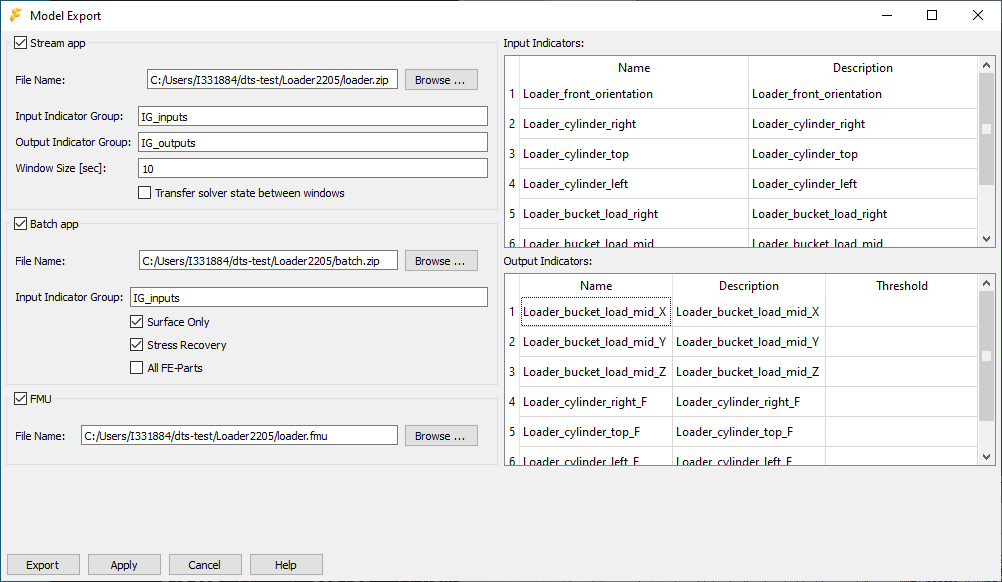
\includegraphics[width=\textwidth]{\ReferenceImg/dlg-model-export}}
    \put(-10, 58){\Bullet{1}}
    \put(-10,118){\Bullet{1}}
    \put(-10,180){\Bullet{1}}
    \put(115, 45){\Bullet{2}}
    \put( 25,167){\Bullet{2}}
    \put( 25,105){\Bullet{2}}
    \put( 65, 93){\Bullet{3}}
    \put( 65,155){\Bullet{3}}
    \put( 75,146){\Bullet{4}}
    \put( 55,137){\Bullet{5}}
    \put( 32,128){\Bullet{6}}
    \put(20,76.1){\Bullet{7}\huge\{}
    \put(200,179){\Bullet{8}}
    \put(203,104){\Bullet{9}}
  \end{picture}
\end{figure}

\begin{bulletlist}
\item
  Activate any of these three toggles to enable the export of the current model
  as a {\sl Stream app}, a {\sl Batch app}, and a {\sl FMU}, respectively.
  The fields in the respective frames will be active only if the associated
  toggle is enabled.

\item{\sl File Name:} --
  For each of the three app types, you can click the \textbf{Browse...} button
  to select the name of the zip-archive that will contain the exported model.

\item{\sl Input Indicator Group:} --
  Specifies the group name of input indicators that will be used in the exported
  {\sl Stream-} or {\sl Batch app}. The names specified here need to be
  reflected in the cloud simulation setup in {\sl EPD Connected Products}.

\item{\sl Output Indicator Group:} --
  Specifies the group name of output indicators that will be used in the
  exported {\sl Stream app}. The name specified here needs to be
  reflected in the cloud simulation setup in {\sl EPD Connected Products}.

\item{\sl Window Size [sec]:} --
  Specifies the length of each time window in seconds for the {\sl Stream app}.

\item{\sl Transfer solver state between windows} --
  Activate this toggle if each time window should be restarted using the final
  state of the previous window as starting point. If not activated,
  each time window will start from the modeling configuration.

\item Toggles for exporting {\sl Batch apps}:
  \begin{itemize}
  \subitem{\sl Surface Only} :
    Activate this toggle to represent all FE parts in the model by surface
    elements only in the visualization model. If not activated,
    the visualization model may be larger since it will also contain internal
    element interfaces (invisible) between the solid finite elements.
  \subitem{\sl Stress Recovery} :
    Activate this toggle to let the app perform deformation- and von Mises
    stress recovery for the FE parts that have the
    {\sl Perform stress recovery during dynamics simulation} toggle enabled in
    the \protect\hyperlink{advanced-tab}{\sl Advanced tab} of
    the Part property editor panel.
  \subitem{\sl All FE-Parts} :
    Activate this toggle to let the app generate a visualization for all
    FE parts in the model. If not activated, only the parts having the
    {\sl Perform stress recovery during dynamics simulation} toggle enabled
    in the \protect\hyperlink{advanced-tab}{\sl Advanced tab} of the Part
    property editor panel will be included in the visualization. When the
    {\sl All FE-Parts} toggle is enabled, FE parts which are not toggled for
    recovery will be represented by their rigid body motion only.
  \end{itemize}

\item{\sl Input Indicators:} --
  This table lists all
  \protect\hyperlink{external-function}{\sl External function}s in the model
  (their {\sl Tag} and {\sl Description}, respectively.
  They will define the content of the named {\sl Input Indicator Group}.

\item{\sl Output Indicators:} --
  This table lists all \protect\hyperlink{functions}{\sl Functions} in the model
  that have the {\sl Use as output sensor} toggle enabled in the property editor
  panel. Their {\sl Tag} and {\sl Description}, respectively, are listed,
  in addition to the description of the {\sl Threshold} settings, if enabled.
\end{bulletlist}

Pressing the \textbf{Export} button will perform the model export for all of the
three app types which have the respective activation toggle enabled.


\SubSection{Solvers tool bar}{solvers-tool-bar}

The \textbf{Solvers} tool bar (shown below) contains the commands to set up and
start each of the mechanism analysis processes, including the post-processing
of individual mechanism parts. The tool bar is organized from left to right
in the order of logical task performance, i.e., the dynamics simulation
(including model reduction, if needed) is performed first,
then the stress recovery, mode shape recovery, and so on.

\begin{figure}[!h]
  \center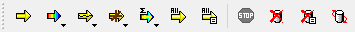
\includegraphics[width=0.6\textwidth]{Figures/6-SolversToolbar}
\end{figure}

The setup commands (\textbf{Dynamics Solver...}, \textbf{Stress Recovery
Setup...}, etc., and \textbf{Additional Solver Options...}) enable management
of all analysis options. Each of the \textbf{Solver} commands are described
in the following sections of this chapter.

\Tip{To access all commands on the \textbf{Solvers} tool bar, click and hold
  down those buttons with an arrow ($\blacktriangledown$) next to the icon.}

\Note{You can also access all Solver tools from the \textbf{Solve} menu.}

\IconText{solveAll}{
  Once you have set up the parameters for each of the solvers you would like to
  execute (as described later in this chapter), click the \textbf{Solve All}
  button on the \textbf{Solvers} tool bar (or from the \textbf{Solve} menu)
  to execute all analyses automatically in consecutive order.}


\SubSection{Additional solver options}{additional-solver-options}

In the Additional Solver Options dialog box, advanced users can fine tune the
behavior of the solver modules through options that are not available elsewhere
from the respective setup dialog boxes or the various Property Editor panels.

\clearpage
\IconText{additionalOptions}{
  Select \textbf{Additional Solver Options...} from the \textbf{Solve} menu
  to open this dialog box (shown below).}

\noindent
\begin{minipage}{0.5\textwidth}
  \raggedright
  \begin{bulletlist}
    \setlength\itemsep{1mm}
  \item
    In each of the first six fields, you may enter text strings of
    command-line options for the respective solver module. Refer to
    \refAppendix{appendix-command-line-options}{Command line options}
    for a complete list of options for all Fedem modules.
  \item
    You can set the maximum number of concurrent processes that will be run
    during a simulation task. This is useful if you have a multi-processor
    machine and want to run several part reductions or recovery processes
    parallel.
  \item
    You can fine-tune the memory usage of the FE model Reducer through
    these options. See
    \protect\hyperlink{optimizing-the-fe-model-reducer-memory-usage}
                      {\sl"Optimizing the FE model Reducer memory usage"}
    below for further details.
  \end{bulletlist}
\end{minipage}% NB: keep this comment
\hfill\begin{minipage}{0.48\textwidth}
  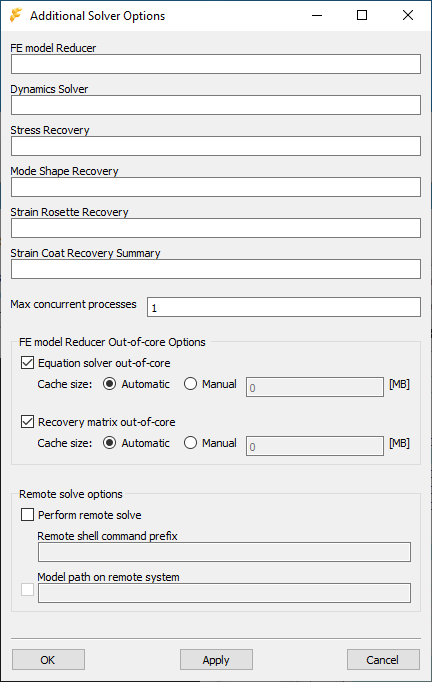
\includegraphics[width=\textwidth]{Figures/Dialogs/6-AdditionalSolverOptions}
  \begin{picture}(-10,-10)
    \put(-175,230){\Bullet{1}}
    \put(-175,215){\Bullet{1}}
    \put(-175,200){\Bullet{1}}
    \put(-175,185){\Bullet{1}}
    \put(-175,170){\Bullet{1}}
    \put(-175,155){\Bullet{1}}
    \put(-175,138){\Bullet{2}}
    \put(-175,118){\Bullet{3}}
    \put(-175,60){\Bullet{4}}
  \end{picture}
\end{minipage}

\begin{bulletlist}
  \setcounter{enumi}{3}
\item
  You can specify a command prefix to be applied on all solve tasks.
  This can be used to launch the simulation tasks on another computer in
  your local network, than the Fedem UI is executed on. See
  \protect\hyperlink{running-solver-processes-on-a-remote-computer}
                    {\sl"Running solver processes on a remote computer"}
  below for further details.
\end{bulletlist}

\Caution{Many of the solver options listed in
  \refAppendix{appendix-command-line-options}{Command line options}
  may already have been provided to the corresponding solver
  through their respective setup dialog boxes. Specifying any such option also
  in the Additional Solver Options dialog box will then override the setting in
  the solver-specific dialog box and should therefore be avoided.}
  %Consult Fedem technical support if you are in doubt
  %on the usage of a particular command-line option.}

\Note{If you mis-spell a command-line option in the Additional Solver Options
  dialog box, or specify options that do not exist, the solver process will run
  as if the invalid options were not specified. A warning for each unrecognized
  option is issued in the \protect\hyperlink{output-list}{\sl Output List} view
  in that case, after the solver process has terminated.}

\SubSubSection{Optimizing the FE model Reducer memory usage}
              {optimizing-the-fe-model-reducer-memory-usage}

Perhaps the most memory critical solve process in Fedem is the FE model
reduction for large models. On 32-bit platforms, the amount of in-core memory
that one process may address is 2 GB (usually the practical limit is lower
due to other processes sharing the same CPU).
In Fedem, a linear equation solver is used in the FE model Reducer which works
out-of-core when necessary. This makes it possible to solve much larger FE
models on a 32-bit platform than would be possible using an in-core solver.
The equation solver reserves an in-core buffer (cache) for the numerical data
of a certain size, and goes out-of core only when this buffer is not large
enough. The performance of the equation solver depends on the size of this
buffer and it may therefore be optimized by fine-tuning this size.

\begin{wrapfigure}[5]{r}{0.45\textwidth}
  \vspace{-4mm}
  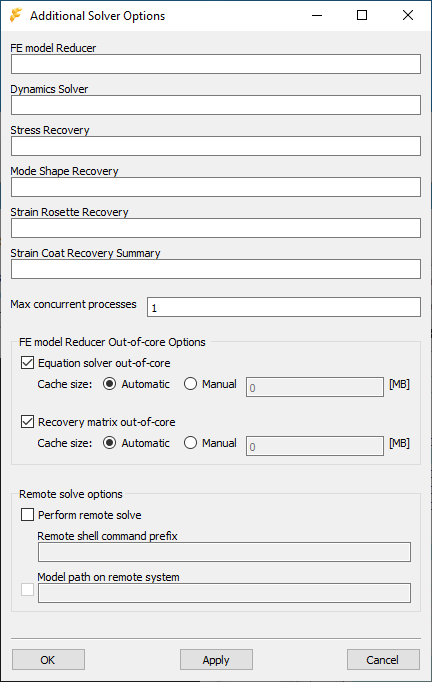
\includegraphics[trim=0 155 0 245,clip,width=0.45\textwidth]
                  {Figures/Dialogs/6-AdditionalSolverOptions}
\end{wrapfigure}

The default is to let the Reducer automatically set the size of the in-core
buffer (as shown to the right). It then reserves a fixed percentage of the free
memory currently available (the actual size is written to the \File{.res} file).
This size may be overridden by switching to {\sl Manual} and entering
the desired cache size in the corresponding field.

You may also switch off the out-of-core feature completely by toggling off the
{\sl Equation solver out-of-core} option.
The Reducer will then abort if the problem does not fit in core.

There is also a similar set of memory usage options that affects the
displacement recovery matrix, and they work in a similar way. Using the
{\sl Manual} setting here corresponds to the {\tt-Bramsize} command-line option.

\Note{Since Fedem R7.2, only the in-core equation solver has been available
  in the FE model Reducer. The out-of-core equation solver settings discussed
  above will therefore be ignored, whereas the options for the recovery matrix
  still apply. The documentation of the out-of-core equation solver settings
  is still retained here for completeness. The out-of-core feature is anyway
  less relevant on current 64-bit platforms (as opposed to older 32-bit
  platforms), where in-core memory is less limited.}

\SubSubSection{Running solver processes on a remote computer}
              {running-solver-processes-on-a-remote-computer}

If you are using a workstation connected to a file server in a local
network together with other computers, it may be advantageous to perform
the simulation tasks on one of the other computers, such that the local
workstation can allocate its resources fully to the Fedem UI process.

\begin{wrapfigure}{r}{0.4\textwidth}
  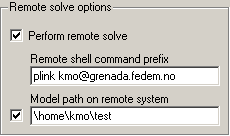
\includegraphics[width=0.4\textwidth]{Figures/6-RemoteSolveOptions}
\end{wrapfigure}

To enable such remote solving, use the {\sl Perform remote solve} toggle in the
{\sl Remote solve options} part of the Additional Solver Options dialog box
(shown to the right). Enter the appropriate {\sl Remote shell command prefix}
needed to run the solver command on the remote computer, and optionally the
{\sl Model path on remote system}.
The latter is necessary when, e.g., your local workstation is a Windows PC and
the remote computer is a UNIX machine. You will then need to specify the path to
the current model file, as it looks from the UNIX computer.

\Caution{When specifying a remote shell command prefix, the input files needed
  by the solver tasks are still created locally within the Fedem UI and not
  explicitly copied on to the remote computer. Thus, a remote execution will
  work only if the local and remote computers use a shared file system.
  Similarly, it is assumed that the Fedem UI on the local computer can access
  the output files created by the solver task directly
  from where they are written by the remote computer.}

\Note{A server program accepting remote shell commands must be running on the
  specified remote computer for this feature to work (e.g., sshd or rshd).
  If using ssh (or the equivalent windows client program plink), you will also
  need to define proper identification keys in your login directory such that
  you can access the remote computer without being prompted for a password.
  Please ask your system operator for assistance on such issues.
  For further information on the ssh and PuTTY/plink programs,
  you may consult the web sites \href{https://www.openssh.com}{openssh.com}
  and \href{https://www.chiark.greenend.org.uk/~sgtatham/putty}
  {chiark.greenend.org.uk/{\textasciitilde}sgtatham/putty}, respectively.}


\SubSection{Controlling placement of temporary files}{controlling-tmp-files}

Some of the Fedem solvers use temporary files during computations, which
are automatically deleted upon completion of the process.

On UNIX systems, these files are placed in the directory pointed to by the
environment variable {\tt TMPDIR}, if set. If {\tt TMPDIR} is not set or points
to a non-existing directory, they are placed in the directory \File{/var/tmp}
instead. On Windows, they are placed in the directory pointed to by the
environment variable {\tt TMP}, if set. If {\tt TMP} is not set or points to a
non-existing directory, they are placed in the directory
\File{C:\textbackslash} instead.

\Note{Some of the temporary files may become very large.
  Make sure that the {\tt TMP} or {\tt TMPDIR} variable
  points to a directory with sufficient amount of free disk space.}


\SubSection{Part- and group-wise solving}{part-and-group-wise-solving}

Fedem has the capability of running some of its solvers on individual
parts of the mechanism (FE Parts and element groups). This is beneficial
when dealing with big models where the solver execution may be both
time- and disc space consuming.

\Note{These solver tasks act upon each part independently, and do not affect
  the global response in any way. The user is encouraged to identify critical
  parts of the model and recover just the results he/she wants on these parts.
  Be aware that each time you recover results they are added to the result
  database, regardless of their previous existence.}

\SubSubSection{Part-wise solving}{part-wise-solving}

\noindent
\begin{minipage}{0.45\textwidth}
  \raggedright
  Solver processes that may be run on parts individually are: Linear Analysis,
  Reducer, Stress recovery, Strain Rosette recovery and Strain Coat recovery.
  A part-wise solve process is started by right-clicking on a Part in the
  {\sl Objects} list of the Model Manager panel, choosing \textbf{Solve},
  and then the wanted process (see illustration to the right).
  You may also multi-select parts in the {\sl Objects} list to solve for two or
  more parts simultaneously. As always, when trying to run the Reducer,
  a part will only be reduced if necessary.
\end{minipage}%
\hfill\begin{minipage}{0.5\textwidth}
  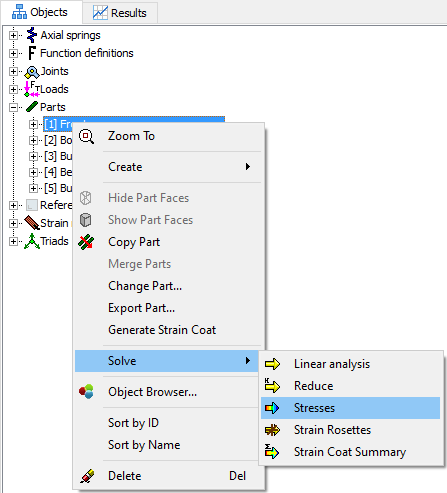
\includegraphics[width=\textwidth]{Figures/6-LinkwiseSolve}
\end{minipage}

\clearpage

\subsubsection{Group-wise solving}

\noindent
\begin{minipage}{0.47\textwidth}
  \raggedright
  Solver processes that may be run on individual element groups are:
  Stress recovery and Strain Coat recovery.
  A group-wise solve process is started in a manner similar to that of
  a part-wise process (see illustration to the right). Right-click
  the group for which you want to solve and then choose the wanted process.
  Multi-selection is possible to solve for two or more groups simultaneously.
  For further information on element groups, refer to
  \refSection{element-groups}{Element groups}.
\end{minipage}%
\hfill\begin{minipage}{0.5\textwidth}
  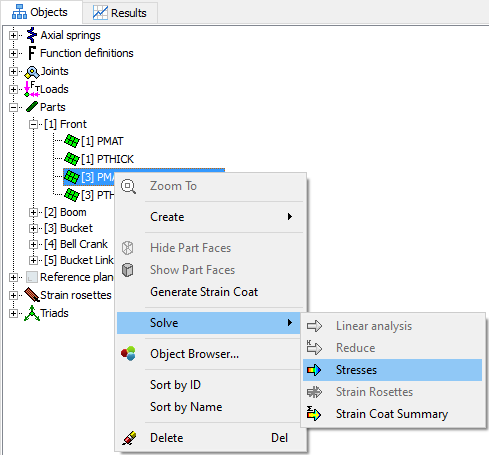
\includegraphics[width=\textwidth]{Figures/6-GroupwiseSolve}
\end{minipage}

\Note{When running Strain Coat recovery on individual parts or element groups,
  a set of strain coat elements are automatically created on all shell and solid
  elements in the current selection, unless such elements have been created in
  a previous run (see also
  \refSection{strain-coat-recovery-on-element-groups-or-individual-parts}
             {Strain coat recovery on element groups or individual parts}).}

\Note{When solving on individual parts or element groups,
  the current settings in the corresponding solver setup dialog box are used.}


\SubSection{Viewing the progress of long-duration analyses}{viewing-progress}

When solving a large model that takes a considerable amount of time, it
is often informative to know exactly how far in the simulation process
we have reached at any time. This can be done simply by viewing a
res-file that is continuously being written by the running solver in the
Result File Browser (see \refSection{result-file-browser}{Result File Browser}).
When such a res-file is selected,
the Info view is automatically scrolled to the bottom of the file
and then continuously updated as the file is being written by the solver.

\Tip{For the model reduction and all of the recovery processes,
  a dedicated progress file called \File{progress\_info.res} is created.
  This file is updated more frequently than the conventional res-file associated
  with the process. Viewing this file while the solver is running will therefore
  give you the best update on its progress.}

\clearpage
It is often wise to also keep an eye on the {\sl Output List} view
while a solver process is running, as important messages produced by the
solver (errors, warnings and notes) are written here while the process
is running (see also
\refSection{how-to-read-error-messages-from-the-solvers}
           {How to read error messages from the solvers}).
All such messages are also written to the res-file, but in the {\sl Output List}
they are prefixed by the solver name and the process ID in brackets, e.g.

\begin{figure}[!h]
  \hskip-0.27\textwidth
  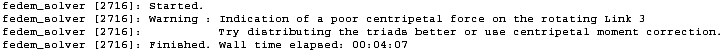
\includegraphics[width=1.27\textwidth]{Figures/6-SolverMessages}
\end{figure}

The first message of a solver process is always {\tt Started.}
and the last message is {\tt Finished.} followed by the consumed wall time.
The process ID number is used to distinguish messages from possibly multiple
simultaneously running reduction or recovery processes.


%%%%%%%%%%%%%%%%%%%%%%%%%%%%%%%%%%%%%%%%%%%%%%%%%%%%%%%%%%%%%%%%%%%%%%%%%%%%%%%%
\Section{Model reduction}{model-reduction}

The FE model reduction process requires no user setup apart from the settings
found in the \protect\hyperlink{reduction-options-tab}
{\sl Reduction Options tab} of the Property Editor panel for each part
(see \refSection{part-properties}{Part properties}).
Some of these options are discussed in further detail in the sub-sections below.


\SubSection{Starting the model reduction}{starting-the-model-reduction}

Model reduction is performed automatically for the parts needing it when you
start the dynamics simulation. Fedem determines automatically which parts need
to be reduced based on the triad configuration and the connection to the rest
of the model. It also checks whether any of the settings in the
\protect\hyperlink{reduction-options-tab}{\sl Reduction Options tab},
that affect the results have been changed since the last reduction of that part.

\vskip\parskip
\IconText{reduceAll}{
  You can also initiate the model reduction process manually at any time.
  Simply select \textbf{Reduce All FE Parts} from the \textbf{Solve} menu
  to do this. You may also initiate the model reduction for only one,
  or a selection of parts, by using the
  \protect\hyperlink{part-wise-solving}{\sl Part-wise solving} command
  (see \refSection{part-and-group-wise-solving}{Part- and group-wise solving}).}

\Note{If element calculations fail during model reduction due to bad element
  shapes, etc., all bad elements in the part are reported before the model
  reduction process exits.}

\Note{Once a part is reduced, it will not be reduced again, even if the
  \textbf{Reduce All Parts} button is clicked again, unless the part has been
  modified in the meantime (by for instance, adding or removing external nodes
  or altering the material properties).}


\SubSection{Using component modes}{using-component-modes}

Fedem uses a Component Mode Synthesis (CMS) model reduction method that
replaces the internal nodal DOFs with a set of static and component modes.
The static modes corresponds to the external nodal DOFs (i.e., at the Triads
attached to the part), whereas the component modes are calculated as the
eigenmode shapes of the part with all external nodes fully constrained.

Component modes describe the internal vibrations in the part. You should
normally include a sufficient number of modes such that the frequencies within
the time step size used in the dynamics simulation are covered.
The frequencies of the computed component modes are found in the output file
\File{fedem\_reducer.res} and can be viewed using the {\sl Result File Browser}
(see \refSection{result-file-browser}{Result File Browser}).

The number of component modes is specified in the Property Editor panel
for the selected part (see
\refSubSection{reduction-options-tab}{Reduction Options tab}{part-properties}.
The default is 0 (no component modes), i.e., only static modes are used.
If the internal vibrations are not important for the overall response,
you can save computation time by using static modes only.
More details on component modes and CMS model reduction can be found in the
\FedemTGuide{Section 3.2, "Component mode synthesis reduction"}.


\SubSection{Using lumped mass matrix}{using-lumped-mass-matrix}

To increase the computational efficiency of the model reduction process,
a lumped mass matrix approach is used by default. The FE mass matrices are then
represented by one diagonal matrix each, where each diagonal term is the sum of
the associated row (or column) of the corresponding consistent mass matrix.
The assembled mass matrix of the part will then also be diagonal, except for
some off-diagonal terms created by the constraint equations\footnote{
You have constraint equations in the part if it contains RBAR, RGD, WAVGM
(RBAR, RBE2, RBE3 in Nastran terminology) and/or BEAM elements with end release.
Thus, as the number of such elements in the part increases, the advantage of
using lumped mass will decrease.}, if any.
Using lumped mass may reduce the memory requirements significantly compared to
using a consistent mass matrix, and also speed up the reduction process as some
of the linear algebra operations involved then are simplified.

\Note{To some degree, using lumped mass does affect the results,
  as it represents a simplification of the FE model.
  The result difference may be significant for parts with a coarse FE mesh.
  However, as the mesh is refined, the difference becomes smaller.
  Therefore, we recommend to use consistent mass on parts not having
  a sufficiently fine mesh. If you are in doubt, do a test run using both
  consistent and lumped mass and compare the results.}

The use of consistent mass matrix is toggled On/Off for the selected part
through a button in the Property Editor panel (see
\refSubSection{reduction-options-tab}{Reduction Options tab}{part-properties}.
The default is {\sl Off} for new parts imported into a model.


\SubSection{Handling singularities during the model reduction}
           {handling-singularities-during-the-model-reduction}

In complex FE modeling, it is inevitable not to have one or more defects in the
FE model from time to time. In the model reduction process, this will typically
result in a singular mass and/or stiffness matrix. Fedem recognizes two types of
singularities, which are handled slightly different in the matrix
triangularization (factorization):

\begin{itemize}
\item
  DOFs that have not received any stiffness/mass contribution at all and
  thus have an exact zero pivot before the triangularization is started,
  are detected {\sl a priori.} The zero pivot is then replaced by the value 1.0,
  which implies that the singular DOF is constrained to zero.
\item
  DOFs that initially have a non-zero pivot, but are reduced to a value
  close to zero during the triangularization, will receive some small
  value on the diagonal, allowing the triangularization process to continue.
  The judgment on whether such singularities have occurred is based on
  the user-provided \protect\hyperlink{singularity-tolerance}
  {\sl Singularity tolerance} (see below).
\end{itemize}

When the reduction process has terminated, a list of all singularities
is written to the {\sl Output List} and the \File{.res} file.
Each singular DOF is here identified by the node ID and local DOF number.
If only singularities of the first kind are detected, the reduction process
completes successfully and it should be safe to use this part in a dynamics
simulation. However, if one or more singularities of the second kind are
detected, the reduction is aborted with no results, and the FE model has to be
manually fixed before continuing.

\Caution{If more than one singularity of the second kind are detected, there is
  a possibility that some of them, except the first one, are fictitious.
  On the other hand, there is also a possibility that not all singularities
  are detected. Thus, after having fixed all the reported singularities
  manually, other singularities may be revealed in the next run.
  This behavior is due to the insertion of a small value on the diagonal which
  actually changes the mechanical property of the FE model.}

It is possible to switch off the above treatment of singularities during
model reduction. This is done by specifying \File{-singularityHandler 0}
as an additional option to the FE model Reducer (see
\refSection{additional-solver-options}{Additional solver options}).
Only the first occurring singularity, regardless of its kind,
will then be reported, and the reduction process will abort immediately.

\SubSubSection{Singularity tolerance}{singularity-tolerance}

The criterion used to determine if a stiffness or mass matrix is
singular during the reduction is specified through a threshold value in
the Property Editor panel for the part (see
\refSubSection{reduction-options-tab}{Reduction Options tab}{part-properties}.
The default value is $1\times10^{-12}$. If the ratio between the current and
previous value of a diagonal matrix element becomes less than the threshold
during the factorization, the matrix is assumed to be singular.

The default threshold value is usually sufficient for well-conditioned
FE models. However, there might be situations where you have a natural high
ratio between the stiffness (or mass) properties in different parts of a model.
In this case you may need to reduce the value to avoid a false error exit.
If you do get a singularity exit but is quite sure your model is sane (although
not that well-conditioned), you should check the actual diagonal decay value
which is written in the \File{.res} file.
You may then try changing the {\sl Singularity criterion} to a value less than
this value and rerun the model reduction.
Note that the lowest admissible value is $1\times10^{-20}$.
Any value lower than that will be ignored and $1\times10^{-20}$ will be used.

\subsubsection{Negative pivots}

A model reduction may also reveal negative pivot elements in the stiffness- or
mass matrix. This may happen if, e.g., the part contains several poorly shaped
elements (especially shell elements).
However, since the linear equation solver is able to handle negative definite
matrices the reduction is not aborted when only negative pivots are encountered.
Nevertheless, it is good practice to go over the FE model once again and check
for bad elements if you get warnings on negative pivots.

\Warning{Using a reduced part with many negative pivots in its stiffness matrix
  may lead to instabilities in the subsequent Dynamics simulation, and should
  therefore be avoided. Only a few negative pivots in a large part is normally
  not a problem, however. That has at most only local influence on the results
  in the vicinity of the elements with the negative pivots.}


\SubSection{Eigenvalue analysis of the reduced parts}
           {eigenvalue-analysis-of-the-reduced-parts}

To assess the dynamic properties of the reduced FE part matrices,
you can perform an eigenvalue analysis of the reduced system, i.e.
$$\left({\bf K} - \omega^2{\bf M}\right)\mbox{\boldmath$\phi$} = {\bf 0}$$
where \textbf{K} and \textbf{M} denote the reduced stiffness and mass matrices.
Since the reduced system does not include any constrained DOFs\footnote{
DOFs that should be constrained are retained during the part reduction and are
constrained only during the system analysis by the dynamics solver.},
the first six eigenvalues should always be zero. The remaining eigenvalues
can then be used to assess the dynamic properties of the reduced part.

The $n$ lowest eigenfrequencies, i.e., the quantities
$$\frac{\omega_i}{2\pi}, \; i = 1 \ldots n $$
for each reduced part can be written to the corresponding \File{.res} file
by specifying \File{-nevred n} in the {\sl FE model Reducer} field in the
Additional Solver Options dialog (see
\refSection{additional-solver-options}{Additional solver options}).
The eigenfrequencies are presented in Hertz.
The default value of this option is 12 for all parts,
but it is not effective for massless parts.
For other parts, the option may be turned off by specifying \File{-nevred 0}.


\SubSection{Visualization of eigenmode shapes from the model reduction}
           {visualization-of-eigenmode-shapes-from-the-model-reduction}

To further verify the results of the reduction process and to increase
the understanding of the part's dynamics properties, it is often useful
to visualize the computed mode shapes of the part.
This is possible if you toggle on {\sl Expand mode shapes} in the
\protect\hyperlink{reduction-options-tab}{\sl Reduction Options tab}
of the Property Editor panel for the parts in question, before they are reduced
(see \refSection{part-properties}{Part properties}).
Both the component mode shapes
(see \refSection{using-component-modes}{Using component modes})
and the mode shapes associated with the eigenvalues of the reduced system
(see \refSection{eigenvalue-analysis-of-the-reduced-parts}
{Eigenvalue analysis of the reduced parts}) will then be computed during the
model reduction, and be subsequently available for viewing in an Eigenmode
animation
(see \refSubSection{eigen-modes-tab}{Eigen Modes tab}{animation-properties}.

\Tip{It is particularly useful to study the mode shapes of the reduced system,
  if for instance more than six modes with (close to) zero eigenfrequency occur.
  That is usually due do an internal mechanism in the model caused by an error
  in the model, and can be revealed if animating the corresponding mode shape.}

\Tip{If you get less than the required six zero rigid mode modes in the reduced
  system for a part, that can be caused by some over-constraining in the
  FE model (e.g., due to bad modeling). By animating the six first mode shapes
  you can then see which rigid body modes are present and which are not,
  and also see the mode shapes that replaced the missing rigid body modes.
  This might give you some hints towards the actual model error or weakness.}


\SubSection{Reduction of applied load vectors}
           {reduction-of-applied-load-vectors}

Along with the reduced mass- and stiffness matrices, the FE model
Reducer always computes reduced (unit) gravity load vectors of the part,
which are applied as a constant static load in the direction of the
defined gravitation vector in the dynamics simulation.

In addition, a set of load vectors corresponding to defined load cases
in the FE data file are computed, when such load definitions are present.
This includes both concentrated point loads and distributed surface loads
on shell and solid elements.

These reduced load vectors may then be assigned time history scaling functions
in the Property Editor panel before the dynamics simulation is run
(see \refSubSection{reduced-loads-tab}{Reduced Loads tab}{part-properties}.


%%%%%%%%%%%%%%%%%%%%%%%%%%%%%%%%%%%%%%%%%%%%%%%%%%%%%%%%%%%%%%%%%%%%%%%%%%%%%%%%
\Section{Model reduction in Nastran}{model-reduction-in-nastran}

As an alternative to the Fedem Model Reduction, the model reduction may
also be performed in Nastran. Nastran supports a similar CMS reduction
procedure as in Fedem, and is able to export the reduced mass- and
stiffness matrix as binary files that may be imported into Fedem. The
advantage of doing the model reduction in Nastran is that you then have
a broader range of element and material properties available for use on
the part level, such as orthotropic materials, composites, etc.


\SubSection{Nastran DMAP}{nastran-dmap}

The Nastran model reduction is performed using a DMAP script to facilitate the
generation of the reduced matrices needed in Fedem.
A Nastran DMAP is a script program (kind of API and programming language)
that modifies the execution of the Nastran solver. The script is model
independent and must be included in the Nastran bulk data file when Nastran
reduction is desired. The script, called \File{nastran\_dmap.dat},
is located in the Template folder of the Fedem installation. Refer to
the Nastran documentation for further details on the DMAP script language.


\SubSection{Nastran bulk data entries for CMS reduction}
           {nastran-bulk-data-entries-for-cms-reduction}

The Nastran bulk data file must contain some commands, in addition to
the entries describing the FE model itself, when it is going to be
reduced in Nastran. Before the CEND keyword, the following commands must
be added to define the output files, solution type and the DMAP script:

\begin{itemize}
\item
  Define OP2-files used to store the reduced mass (m), stiffness (s) and
  gravity (g) matrices from Nastran (\textless name\textgreater{} is
  here some arbitrary string identifying this part):

  \texttt{%
    ASSIGN, output2=\textquotesingle\textless name\textgreater\_m.op2\textquotesingle, UNIT=71 \\
    ASSIGN, output2=\textquotesingle\textless name\textgreater\_s.op2\textquotesingle, UNIT=72 \\
    ASSIGN, output2=\textquotesingle\textless name\textgreater\_g.op2\textquotesingle, UNIT=73}
\end{itemize}

\Note{The OP2-files are automatically converted to \File{.fmx} files
  when the Nastran bulk data file is imported into Fedem,
  and the part is recognized as {\rm Reduced}.}

\begin{itemize}
\item Specify modal analysis: \\
  \texttt{SOL 103}
\item Include DMAP script: \\
  \texttt{INCLUDE \textquotesingle nastran\_dmap.dat\textquotesingle}
\end{itemize}

After the \texttt{BEGIN BULK} keyword, the following commands must be added
to perform the Nastran CMS-reduction:

\begin{itemize}
\item If you need to attach triads or joints to shell element nodes,
  you need to turn on the drilling dof on the Nastran shell elements:

  \texttt{PARAM, K6ROT, \textless value\textgreater}

  \textless value\textgreater = 10 or a small value is recommended.
  (If it is set to 0 the drilling dof is omitted, which is not what is desired).
  The value is used to calculate an artificial stiffness that might influence
  the overall stiffness. This might introduce undesirable effects,
  and the resulting component modes should therefore be compared with component
  modes calculated without this artificial stiffness.

\item To get consistent instead of lumped mass representation
  the following bulk data command may be added:

  \texttt{PARAM, COUPMASS,1}

  If coupled mass is not used, the DMAP script can be simplified since
  $M_{ie} = M_{ei} = 0$.

\item Definition of static modes (external dofs).
  Use ASET or ASET1 entries to define the external dofs. To get 6-DOF Triads,
  all nodes in the ASET (active dof set) must have 6 active DOFs.
  A typical bulk entry is:

  \texttt{ASET, node\_id1, 123456, node\_id2, 123456, ...}
\end{itemize}

Adding component modes (generalized dofs)

\begin{itemize}
\item If component modes (generalized dofs) are desired,
  the following bulk entries must be specified:

  \texttt{%
  EIGRL,1,,,\textless idn\textgreater \\
  SPOINT,\textless id1\textgreater,\textless id2\textgreater...\textless idn\textgreater \\
  QSET1,0,\textless id1\textgreater,\textless id2\textgreater...\textless idn\textgreater}

  Here, \textless idn\textgreater is the number of component modes.
\end{itemize}


\SubSection{Recovery of parts reduced in Nastran}
           {recovery-of-parts-reduced-in-nastran}

When the model reduction is performed in Nastran, you also have to perform the
part-level recovery in Nastran. Stress Recovery, Mode Shape Recovery, etc.,
can not be performed by Fedem for such parts.

Some dynamics solver results must be exported to bulk data format files when
part-level recovery is to be performed in Nastran.
To do this, specify {\tt -saveInc3 \textless inc\textgreater} as
\protect\hyperlink{additional-solver-options}{\sl Additional solver options}
for the dynamics solver, where
{\tt\textless inc\textgreater} is the time increment between each time step you
want to perform recovery for. You will then get one file for each
Nastran-reduced part for each time step in the results database.
These files have names on the form
\File{adisp\_\textless part\textgreater\_t\textless istep\textgreater.bdf},
where \File{\textless part\textgreater} is the base name of the FE model file
and \File{\textless istep\textgreater} is the time step number.
They can be loaded into Nastran together with the FE model file for doing
the recovery there.


%%%%%%%%%%%%%%%%%%%%%%%%%%%%%%%%%%%%%%%%%%%%%%%%%%%%%%%%%%%%%%%%%%%%%%%%%%%%%%%%
\Section{Dynamics analysis}{dynamics-analysis}

\IconTextFirst{solve}{
  To control the dynamics analysis parameters,
  click the \textbf{Dynamics Solver} button on the \textbf{Solvers} tool bar (or
  select \textbf{Dynamics Solver (Basic Mode)...} from the \textbf{Solve} menu).
  The Dynamics Solver dialog box (shown below) will then appear, and allow you
  to adjust the simulation setup.}

In-depth information about the time integration algorithm used in the dynamics
solver may be found in the \FedemTGuide{Chapter 7, "Dynamics Simulation"}.


\SubSection{Dynamics Solver (Basic Mode)}{dynamics-solver-basic-mode}

In its basic mode, the Dynamics Solver dialog box contains the following:

\noindent
\begin{minipage}{0.5\textwidth}
  \raggedright
  \begin{bulletlist}
    \setlength\itemsep{1mm}
  \item{\sl Initial equilibrium} --
    Enables a static equilibrium analysis to move the mechanism to a resting
    position before simulating the dynamics, see
    \refSubSection{static-equilibrium-analysis}{Static equilibrium analysis}
                  {dynamics-analysis-overview}.

  \item{\sl Time history response analysis} --
    Enables the dynamics simulation of the time history response,
    with specification of the {\sl Start}, {\sl Stop} and {\sl increment} size
    of the Time domain.

  \item{\sl Quasistatic analysis} --
    Enables a quasi-static simulation, either for the complete time interval
    or up to a given time. In this analysis, all velocity- and acceleration
    terms (i.e., damping and inertia forces and associated tangent
    contributions) are set to zero.
  \end{bulletlist}
\end{minipage}%
\hfill\begin{minipage}{0.45\textwidth}
  \begin{picture}(155,228)
    \put(0,0){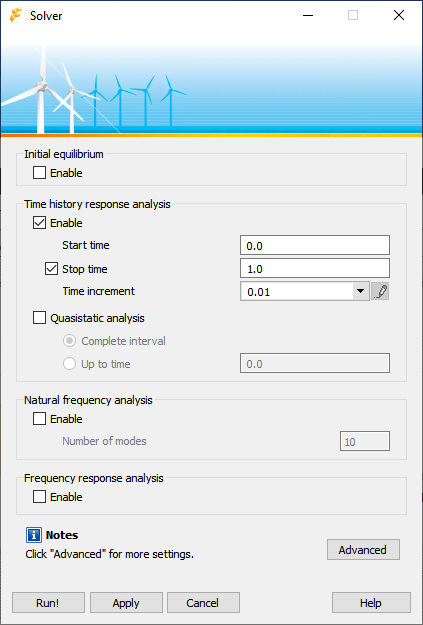
\includegraphics[width=\textwidth]{\ReferenceImg/dlg-solver-basic1}}
    \put(-5,161){\Bullet{1}}
    \put(-5,142){\Bullet{2}}
    \put(-5,107){\Bullet{3}}
    \put(-5, 70){\Bullet{4}}
    \put(-5, 42){\Bullet{5}}
  \end{picture}
\end{minipage}

% Using the more generic macro here instead of \Tip, to get the indentation righ
\MiniGenericNote{tip}{TIP}{-26mm}{1.1}{0.165}{0.835}{
  The {\sl Quasistatic analysis} can be used in place of
  (or in addition to) the {\sl Initial equilibrium} analysis to obtain a proper
  start configuration for the subsequent dynamics simulation, in case the
  modeling configuration is so far off equilibrium that more than
  one load step is needed to obtain a converged configuration.}

\begin{bulletlist}
  \setcounter{enumi}{3}

\item{\sl Natural frequency analysis} -- Enables eigenvalue analysis
  to be performed to compute a specified number of modes, see
  \refSubSection{modal-analysis}{Modal analysis}{dynamics-analysis-overview}.
  The eigenvalue calculation is performed on the initial configuration,
  and then at time intervals as specified in the
  \protect\hyperlink{eigenmode-tab}{\sl Eigenmode tab} of the {\sl Advanced}
  solver dialog box (see \refSection{dynamics-solver-advanced-mode}
  {Dynamics Solver (Advanced Mode)} below).

\item{\sl Frequency response analysis} --
  Enables a frequency response analysis to be performed during the time history
  response simulation, if the model contains Triad- or Joint DOF loads or
  prescribed motions which have been defined as frequency domain inputs, see
  \refSection{triad-properties}{Triad properties} and
  \refSubSection{joint-variable-properties}{Joint variable properties}
                {joint-properties}.
  The toggle is inactive if no such loads or motions exist in the model.

  See \refSection{frequency-response-analysis}{Frequency response analysis}
  for more details on performing frequency response analyses.
\end{bulletlist}

You can click the \textbf{Run!} button to start the dynamics solver, or the
\textbf{Advanced} button, if more specialized setup is needed first (see below).


\SubSection{Dynamics Solver (Advanced Mode)}{dynamics-solver-advanced-mode}

The advanced settings for the Dynamics Solver are placed on six tabs in the
dialog box labeled {\sl Time}, {\sl Integration}, {\sl Tolerances},
{\sl Eigenmode}, {\sl Initial Equilibrium}, and {\sl Output}, respectively,
and are described in the following.

All six tabs have in common that they have a \textbf{Basic} button that will
take you back to the basic mode of the Solver dialog box
(see \refSection{dynamics-solver-basic-mode}{Dynamics Solver (Basic Mode)}).
If you then click the corresponding \textbf{Advanced} button in the basic
Solver dialog box, you will return to the tab that you just left.

\SubSubSection{Time tab}{time-tab}

The time domain of the dynamics simulation is controlled through the
following parameters:

\noindent
\begin{minipage}{0.5\textwidth}
  \raggedright
  \begin{bulletlist}
    \setlength\itemsep{2mm}
  \item
    You can define the {\sl Start time} and the {\sl Stop time} of the
    dynamics simulation.
  \item
    You can define the size of the {\sl Time increment} to be used by the time
    integration algorithm. In addition to a constant value, you may also select
    a {\sl Function} or a {\sl Time history input file} from the pull-down menu,
    in order to obtain a varying time increment size
    (see \refSection{functions}{Functions}).
    In that case, the {\sl Minimum time increment} is used as a lower bound on
    the time step size.
  \end{bulletlist}
\end{minipage}%
\hfill\begin{minipage}{0.45\textwidth}
  \begin{picture}(155,228)
    \put(0,0){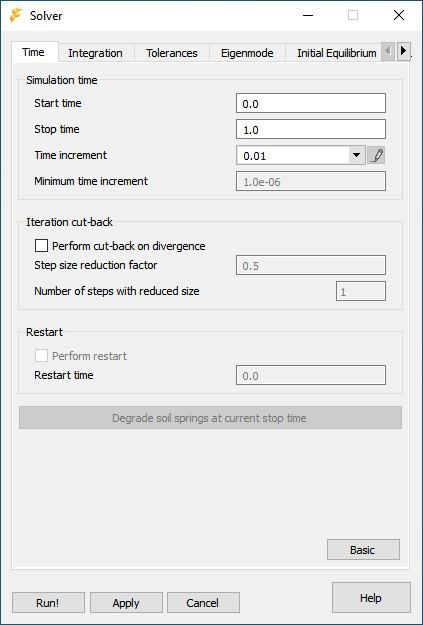
\includegraphics[width=\textwidth]{\ReferenceImg/dlg-solver-advanced1}}
    \put(-4,181){\Bullet{1}}
    \put(-4,162){\Bullet{2}}
    \put(-4,126){\Bullet{3}}
    \put(-4, 94){\Bullet{4}}
  \end{picture}
\end{minipage}

\clearpage
\begin{bulletlist}
  \setcounter{enumi}{2}
\item
  You can enable/disable the use of {\sl Iteration cut-back} when the dynamics
  simulation diverges, and adjust the {\sl Step size reduction factor} defining
  the size of the new time step to use in the cut-back,
  and the {\sl Number of time steps with reduced size}
  before the normal step size is resumed.
  If the cut-back iterations also diverge, another cut-back is attempted
  by applying the {\sl Step size reduction factor} again.
  This procedure is then repeated until convergence is obtained or the
  {\sl Minimum time increment} is reached.
  In the latter case, the simulation is aborted.
\item
  You can enable a {\sl Restart} simulation if you already have some simulation
  results, and specify the {\sl Restart time} defining the time step to restart
  from. If the specified time does not match an existing time step,
  the closest step after the specified time is used.
\end{bulletlist}

\Note{In a restart simulation, you are allowed to adjust any of the other
  Solver Setup parameters and options, as well as adjusting the additional
  solver options for the Dynamics solver
  (see \refSection{additional-solver-options}{Additional solver options}).
  However, you can not change any properties of the mechanism model itself.}

Restarting a Dynamics simulation is very handy if you discover you need
to continue a simulation that was terminated abnormally,
or you just want a longer event than was originally defined.
You may restart a simulation as many times you wish.

Each restart adds a new set of result files to the existing results database
such that subsequent post-processing and recovery runs can be conducted over
the overall time domain spanned by both the initial run and the restart(s).
If the time domain of the individual runs overlap, only the latest produced
results will be used in post-processing and recovery.
See \refSection{result-files-from-restart-simulations}
{Result files from restart simulations} for more information
on the management of results from restart simulations.

\clearpage

\SubSubSection{Integration tab}{integration-tab}

You can optimize numerical performance of the time integration by adjusting the
following parameters:

\noindent
\begin{minipage}{0.5\textwidth}
  \raggedright
  \begin{bulletlist}
    \setlength\itemsep{1mm}
  \item
    You can select between three different time integration algorithms
    ({\sl HHT-alpha} with $\alpha_H = 0.1$ is recommended).
    Refer to the \FedemVer~Theory Guide, Sections 7.2, 7.3 and
    especially 7.4 {\sl"Newmark integration with numerical damping"}
    for details on the different time integration schemes available.
  \item
    You can enable/disable the use of {\sl Integration tolerances},
    and specify the {\sl Maximum} and {\sl Minimum number of iterations}
    for each time increment. When {\sl Ignore integration tolerances} is set,
    the fixed {\sl Number of iterations} is specified instead.
  \end{bulletlist}
\end{minipage}%
\hfill\begin{minipage}{0.45\textwidth}
  \begin{picture}(155,228)
    \put(0,0){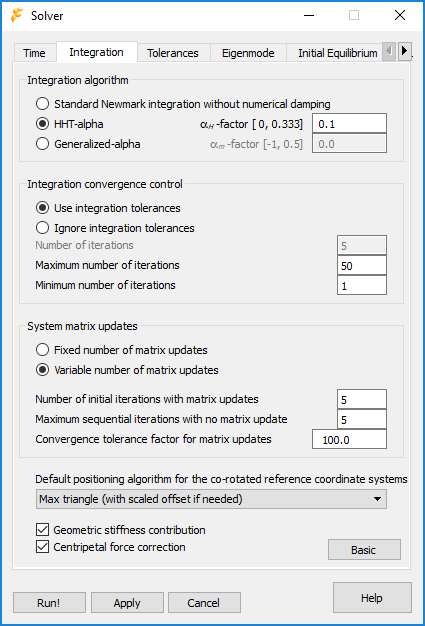
\includegraphics[width=\textwidth]{\ReferenceImg/dlg-solver-advanced2}}
    \put(-4,178){\Bullet{1}}
    \put(-4,143){\Bullet{2}}
    \put(-4, 92){\Bullet{3}}
    \put(-4, 42){\Bullet{4}}
    \put(-4, 26){\Bullet{5}}
  \end{picture}
\end{minipage}

\begin{bulletlist}
  \setcounter{enumi}{2}
\item
  The nonlinear equations are solved using Modified Newton-Raphson iterations
  meaning that the system matrices are not necessarily recalculated in each
  iteration. For efficiency reasons, the number of matrix updates per time step
  should be as low as possible. However, if the increments in the input variable
  s are large during a time step, the system matrices need to be updated more
  often, to ensure the nonlinear iterations converge.

  You may choose between {\sl Fixed number of matrix updates} or
  {\sl Variable number of matrix updates}. In either case you can also specify
  the {\sl Number of initial iterations with matrix updates} and
  the {\sl Maximum sequential iterations with no matrix updates}.
  The first number defines how many iterations in the beginning of each time
  step should be performed with updated matrices. If the iterations have not
  converged before reaching that number, the subsequent iterations are performed
  with a matrix update frequency defined by the
  {\sl Maximum sequential iterations with no matrix updates}.
  However, if {\sl Variable number of matrix updates} is chosen,
  a convergence based threshold is used in addition to determine when to
  do further system matrix updates.
  The factor entered in {\sl Convergence tolerance factor for matrix updates}
  is then multiplied with the active convergence tolerances specified on the
  \protect\hyperlink{tolerances-tab}{\sl Tolerances tab}.
  The resulting tolerance is compared to the error norms corresponding to the
  active convergence tolerances and the matrices are updated
  as long as the error norm is higher than this tolerance.

\item You can specify the default algorithm for
  calculation of the co-rotated part coordinate systems during the simulation.
  The selections available correspond to those of the similar pull-down menu in
  the \protect\hyperlink{advanced-tab}{\sl Advanced tab} of the Property Editor
  panel for Parts (see \refSection{part-properties}{Part properties)}.
  The setting here applies to all parts in the model, where the corresponding
  setting on the part level is {\sl Model default}.

\item You can enable/disable both the
  {\sl Geometric Stiffness Contribution} and the
  {\sl Centripetal Moment Correction} during the non-linear iterations.
  The geometric stiffness option accounts for stress stiffening in parts,
  and axial springs and dampers. It may thus improve the convergence of
  the nonlinear iterations if the model contains parts with large membrane
  forces or axial springs and dampers with large forces. This is because
  the forces alters the bending- or rotational stiffness of these elements.
  A tensile membrane/axial force will effectively increase the
  bending/rotational stiffness and a compressive force will reduce the
  bending/rational stiffness. For information on the computation of the
  geometric stiffness on parts, see the
  \FedemTGuide{Section 4.4, "Superelement tangent stiffness".}

  The centripetal moment correction option enables an improved representation of
  the inertia forces on parts with only a few Triads that experience high-speed
  rotations (see the
  \FedemTGuide{Section 3.3, "Inertia forces and high-speed rotation"}
  for details).
\end{bulletlist}

\clearpage

\SubSubSection{Tolerances tab}{tolerances-tab}

Convergence criteria for the dynamics analysis are defined by enabling one,
or more, convergence tolerances:

\noindent
\begin{minipage}{0.5\textwidth}
  \raggedright
  \begin{bulletlist}
    \setlength\itemsep{1mm}
  \item
    This allows you to define and enable/disable convergence tolerances on the
    {\sl Displacement iteration corrections}.
  \item
    You can define a convergence tolerance on
    {\sl Velocity iteration correction}.
  \item
    You can define various tolerances on {\sl Unbalanced forces (residual)}.
  \item
    You can define tolerances on {\sl Iteration energy changes}.
  \item
    All available convergence tests can be ignored or defined into one of two
    sets of tests: In set {\sl A}, all tests must be satisfied for convergence
    to be satisfied. In set {\sl O}, only one of the tests must be satisfied (in
    addition to all the tests in set {\sl A}) for convergence to be satisfied.
  \end{bulletlist}
\end{minipage}%
\hfill\begin{minipage}{0.45\textwidth}
  \begin{picture}(155,228)
    \put(0,0){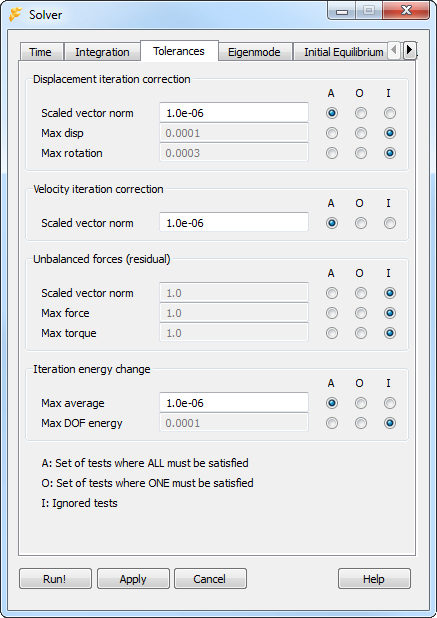
\includegraphics[width=\textwidth]{\ReferenceImg/dlg-solver-advanced3}}
    \put(-3,165){\Bullet{1}}
    \put(-3,135){\Bullet{2}}
    \put(-3,103){\Bullet{3}}
    \put(-3, 67){\Bullet{4}}
    \put(-3, 42){\Bullet{5}}
  \end{picture}
\end{minipage}

\medskip
The various norms used in the above convergence criteria have different
dimension properties. Some are dimensionless, whereas others depend on the model
units. The default values defined are suitable for the SI unit set.
If you model in a different unit set
(see \refSection{model-preferences}{Model preferences}),
you will need to adjust some of your active tolerance values accordingly.

The scaled vector norm of the displacement correction is dimensionless, whereas
the same norm for the velocity correction has dimension 1/[time] and for
the force residual it is [force][length]. The Max norms have the dimension
corresponding to the quantity that they measure.

For more information about convergence criteria,
see the \FedemTGuide{Section 7.3.1, "Convergence criteria"}.

\clearpage

\SubSubSection{Eigenmode tab}{eigenmode-tab}

You can set up the calculation of eigenmode solutions
(see \refSubSection{modal-analysis}{Modal analysis}{dynamics-analysis-overview})
by adjusting the following parameters:

\noindent
\begin{minipage}{0.5\textwidth}
  \raggedright
  \begin{bulletlist}
    \setlength\itemsep{1mm}
  \item This option allows you to
    enable/disable calculation of the eigenmode solutions.
  \item You can specify the number of eigenmodes to be computed.
  \item You can specify the time interval between each eigenvalue analysis.
  \item You can specify an {\sl Eigenmode Shift} (see the \FedemTGuide{
    Section 9.6.3, "Using shift when solving the eigenvalue problem"}).
  \item  You can enable/disable the application of the
    {\sl Additional Boundary Conditions} specified for triads
    (see \refSection{triad-properties}{Triad properties}).
  \end{bulletlist}
\end{minipage}%
\hfill\begin{minipage}{0.45\textwidth}
  \begin{picture}(155,225)
    \put(0,0){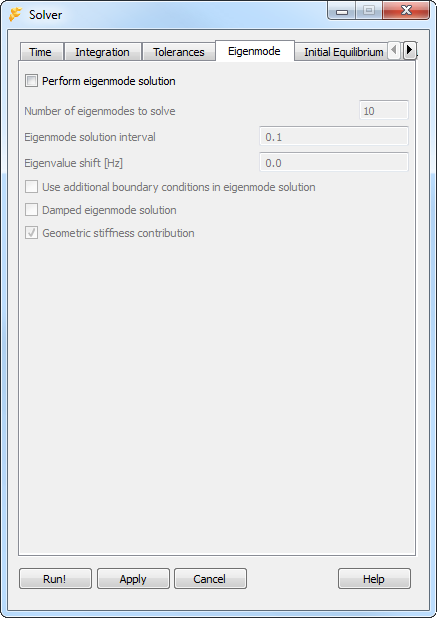
\includegraphics[width=\textwidth]{\ReferenceImg/dlg-solver-advanced4}}
    \put(-6,185){\Bullet{1}}
    \put(-6,175){\Bullet{2}}
    \put(-6,165){\Bullet{3}}
    \put(-6,156){\Bullet{4}}
    \put(-6,148){\Bullet{5}}
    \put(-6,139){\Bullet{6}}
    \put(-6,130){\Bullet{7}}
  \end{picture}
\end{minipage}

\begin{bulletlist}
  \setcounter{enumi}{5}
\item
  You can enable/disable computation of damped eigenmodes by accounting for
  structural damping (see the
  \FedemTGuide{Section 9.6.2, "Damped eigenvalue problem"}).

  \EnumCaution{Computation of damped eigenmodes takes considerably longer time
    than computing the undamped modes.}
\item
  You can enable/disable the {\sl Geometric Stiffness Contribution}
  in the eigenvalue analyses (see the similar option in
  the \protect\hyperlink{integration-tab}{\sl Integration tab}).
  If the mechanism contains structural members that experience large tensile or
  compression forces at certain time steps, the geometric stiffness contribution
  may have a significant effect on the accuracy on the computed eigenvalues
  at those time steps.
\end{bulletlist}

\clearpage

\SubSubSection{Initial Equilibrium tab}{initial-equilibrium-tab}

If, during modeling,
your model is not positioned at its static equilibrium position,
it is recommended that you perform the {\sl Initial Equilibrium} analysis
to move the mechanism to a resting position before simulating the dynamics.

\noindent
\begin{minipage}{0.5\textwidth}
  \raggedright
  \begin{bulletlist}
    \setlength\itemsep{1mm}
  \item
    You can enable this option to perform static equilibrium iterations on the
    modeling configuration.
  \item
    You can adjust the iteration tolerance and the step-size factor for
    the initial static equilibrium iterations.
  \item
    You can enable/disable the {\sl Geometric Stiffness Contribution}
    in initial static equilibrium iterations (see the similar option in the
    \protect\hyperlink{integration-tab}{\sl Integration tab}).
  \item
    You can enable a dynamic load ramp-up simulation, optionally also with
    gravity force ramping, as an alternative (or supplement) to the initial
    static equilibrium analysis.
\end{bulletlist}
\end{minipage}%
\hfill\begin{minipage}{0.45\textwidth}
  \begin{picture}(155,225)
    \put(0,0){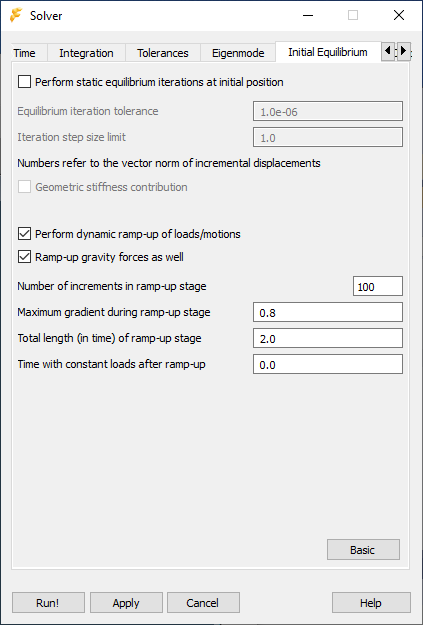
\includegraphics[width=\textwidth]{\ReferenceImg/dlg-solver-advanced5}}
    \put(-9,193){\Bullet{1}}
    \put(-9,178){\Bullet{2}}
    \put(-9,157){\Bullet{3}}
    \put(-9,133){\Bullet{4}}
    \put(-9,118){\Bullet{5}}
    \put(-9,104){\Bullet{6}}
    \put(-9,90){\Bullet{7}}
  \end{picture}
\end{minipage}

% Using the more generic macro here instead of \Tip to get the indentation right
\MiniGenericNote{tip}{TIP}{-26mm}{1.1}{0.165}{0.835}{
  The {\rm dynamic ramp-up of loads/motions} option can be useful if the initial
  loads or motion constraints are too large to be applied in a single static
  step. See \refSection{dynamic-ramp-up-of-loads-and-prescribed-motions}
                       {Dynamic ramp-up of loads and prescribed motions}
  for more information on this.}

\begin{bulletlist}
  \setcounter{enumi}{4}
\item
  You can specify the number of time steps of the ramp-up simulation.
\item
  You can specify the maximum gradient of the scaling function and the
  total length (in time) of the ramp-up simulation stage. The time
  increment size of the ramp-up stage will then be set equal to the
  total length divided by the specified number of time steps.
\item
  You can specify a time for which the loads will be kept constant after
  completed ramp-up stage, before the actual load history is applied.
  This can be used to allow the state approaching a steady state with
  smaller velocities/accelerations, before starting the real dynamics.
\end{bulletlist}

\clearpage
The {\sl Equilibrium iteration tolerance} is the convergence criterion on the
norm of the iterative displacement correction during the initial static
equilibrium iterations (equivalent to the {\sl Scaled vector norm} tolerance
for {\sl Displacement iteration correction} in the
\protect\hyperlink{tolerances-tab}{\sl Tolerances tab}).

The {\sl Iteration step size limit} is an upper limit on the norm of the
displacement correction vector within one iteration. If the norm is higher than
this value, the correction vector is scaled down such that its norm equals this
number. Each time this happens, the iteration counter that is compared to the
{\sl Maximum} and {\sl Minimum Number of Iterations} parameters of the
\protect\hyperlink{integration-tab}{\sl Integration tab}, is reset to zero.

\Note{Maximum and Minimum Number of Iterations set in the
  \protect\hyperlink{integration-tab}{\sl Integration tab}
  also apply in the Initial Equilibrium analysis.}

\Tip{The defaults for the Equilibrium Iteration Tolerance and Iteration
  Step-Size Factor are usually acceptable. However, if the mechanism is
  modeled far from the equilibrium position, reducing the Iteration
  step-size limit may improve performance.}

\Caution{The Iteration step size limit must always be larger than the
  Equilibrium Iteration Tolerance.}

\Caution{To perform the initial equilibrium analysis, you may have to apply
  {\rm Additional Boundary Conditions} before starting the simulation.
  (For information about applying such boundary conditions, see
  \refSection{triad-properties}{Triad properties}.)}

\clearpage

\SubSubSection{Output tab}{output-tab}

On this tab you can control the automatic curve and animation export from
the Dynamics Solver to file. The automatic curve export is useful if you want
to run Fedem in an iterative loop with some external software, and need to
process selected solver output in order to calculate new input for subsequent
runs. The automatic animation export writes a GLview VTF-file with the rigid
body motion of the computed response.
This file may then be opened in the Ceetron GLview software for further viewing
(see \href{https://www.ceetron.com}{ceetron.com} for further details on GLview).

\noindent
\begin{minipage}{0.5\textwidth}
  \raggedright
  \begin{bulletlist}
    \setlength\itemsep{1mm}
  \item
    This toggle enables export of all curves in the model with
    {\sl Export curve automatically} toggled on the property Editor panel
    (see \refSection{curve-properties}{Curve properties}).
  \item This field shows
    the path and name of the file the curve data will be written to.
    Press \textbf{Browse...} to change file name or file format.
  \item
    This label shows the selected format for the curve export.
    Available formats are MTS RPC (UNIX or PC formatting),
    and tab-separated multi-column ASCII.
  \end{bulletlist}
\end{minipage}%
\hfill\begin{minipage}{0.45\textwidth}
  \begin{picture}(155,215)
    \put(0,0){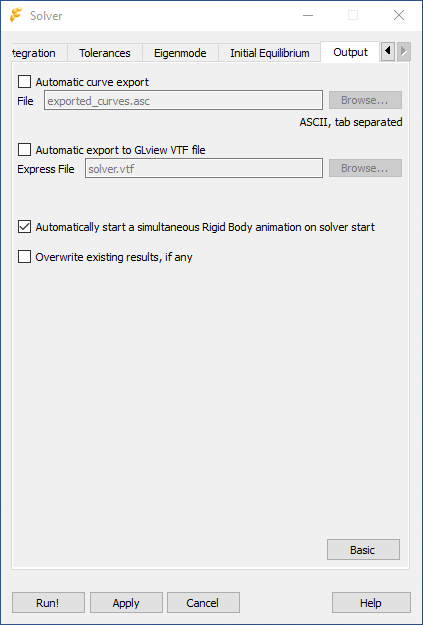
\includegraphics[width=\textwidth]{\ReferenceImg/dlg-solver-advanced6}}
    \put(-8,194){\Bullet{1}}
    \put(105,188){\Bullet{2}}
    \put( 96,177){\Bullet{3}}
    \put(-8,168){\Bullet{4}}
    \put(105,161){\Bullet{5}}
    \put( 9,153){\Bullet{6}}
    \put(-8,141){\Bullet{7}}
    \put(-8,130){\Bullet{8}}
  \end{picture}
\end{minipage}

Only curves plotting results produced by the Dynamics Solver can be exported
in this manner. If you need to include curves with results from other Fedem
simulations in the same output file (e.g., results from subsequent strain
rosette analyses), you have to run the Fedem Curve Export Utility module instead
(see \refSection{automated-curve-export-from-multiple-result-database-files}
                {Automated curve export from multiple result database files}).

\begin{bulletlist}
  \setcounter{enumi}{3}
\item
  This toggle enables export of the rigid body motion of the computed
  response to a GLview VTF-file.
\item
  This field shows path and name of the VTF-file that will be written.
  Press the \textbf{Browse...} button to change file name or file
  format.
\item
  This label shows the selected VTF file format. Available formats are
  Express, Binary and ASCII.
\item
  You can enable/disable the automatic start of a simultaneous rigid
  body animation when the Dynamics Solver is started. This is useful
  when doing rapid prototyping simulations of short duration, when it is
  essential to get quick feedback on the dynamic response.
\item
  You can enable/disable {\sl Overwrite existing results, if any},
  such that you do not have to delete the existing results before
  starting the Dynamics Solver. Instead, the result files are overwritten
  and no incrementation of the results database is performed.
  This means that the old results are lost, even if you close the model
  without saving after a simulation.
\end{bulletlist}

\Caution{When the automatic VTF export is enabled,
  the FE data for all parts in the model is written to the specified VTF file
  before the Dynamics Solver is started.
  For large models this may take some time (especially if the FE data is
  unloaded), and the Fedem UI is blocked while the FE data is being exported.}


\SubSection{Frequency response analysis}{frequency-response-analysis}

In some cases there might be input loads (or prescribed motions) in a
mechanism which have variations over the time span of the simulation
that makes it inconvenient to represent them in a direct time integration.
It would require a very small time step size to resolve the load variation
properly. In such cases the loads are better accounted for by considering them
in the frequency domain instead of the time domain.

This is done by performing a {\sl Fast Fourier Transform (FFT)} of each load
function, resulting in a frequency-dependent load magnitude function, instead of
a time-dependent function. The dynamics equation of motion is then transformed
into the frequency domain and solved for a suitable range of driving
frequencies. The frequency-dependent response can then be transformed back into
the time domain through an inverse FFT, and optionally added to the response of
other time-dependent loads.
See the \FedemTGuide{Section 7.9, "Frequency Response Analysis"}
for the theoretical foundation of the frequency response analyses.

A Frequency response analysis is activated in Fedem through a toggle in
the basic Dynamics Solver Setup dialog box, see
\refSection{dynamics-solver-basic-mode}{Dynamics Solver (Basic Mode)}.
In addition, you may need to specify some additional options for the Dynamics
Solver (see \refSection{additional-solver-options}{Additional solver options})
in order to control the frequency response analysis.
These solver options are listed in the table below.

\noindent
\begin{tabular}{ | m{22mm} | m{9cm}| }
  \hline{\tt-sample\_freq} &
  Sampling frequency [Hz] of the input loads to be used in the FFT calculation.
  The default value is 100 Hz. \\

  \hline{\tt-windowSize} &
  Number of samples in each window in a segmented analysis.
  The default value is zero, meaning the entire time domain of the analysis
  is considered a single window (no segmenting). \\

  \hline{\tt-nrModes} &
  Number of eigenmodes to use in a modal frequency response analysis.
  The default value is zero, which means a direct frequency response analysis
  is used. \\
  \hline
\end{tabular}

The results of the frequency response analysis is stored on a separate
\File{.frs} file in the results database, typically named \File{fd\_p\_\#.frs},
where the \File{\#} character represents a number.
You may then plot the response from the frequency response analysis by
activating this file in the results file browser (see
\refSection{result-manipulation}{Result manipulation}),
while deactivating the other \File{.frs} files generated by the Dynamics Solver.


\SubSection{Dynamic ramp-up of loads and prescribed motions}
           {dynamic-ramp-up-of-loads-and-prescribed-motions}

Sometimes you may want to start the dynamics simulation of a mechanism from a
certain load or motion stage which is far from the modeling configuration.
Ideally, you would like to apply this load/motion state by activating the
{\sl static equilibrium iterations} toggle in the
\protect\hyperlink{initial-equilibrium-tab}{\sl Initial Equilibrium tab},
but this may fail due to that the loads are too large to be applied in one go,
and/or the mechanism is singular such that a static analysis is not possible.

The {\sl Perform dynamic ramp-up of loads/motions} option is a tool which may be
used instead in such cases. It will perform a dynamics (or quasi-static)
simulation over a specified time range (from $t=t_0-T$ to $t=t_0$, where $t_0$ is
the start time specified in the \protect\hyperlink{time-tab}{\sl Time tab},
and $T$ is the total length of the ramp-up stage).
In this simulation stage, all external loads and prescribed motions in the model
that are functions of time, will be evaluated at $t=t_0$ and then scaled with
a time-dependent smooth ramp function to obtain the load level that should be
applied at a certain time. Optionally, the gravity loads may be scaled with the
ramp function as well (although this is usually not necessary).

The scaling function that is used in the ramp-up simulation is a
\protect\hyperlink{smooth-trajectory}{\sl Smooth trajectory} function
(see \refSection{function-properties}{Function properties}),
which is defined by the following three parameters:

\begin{itemize}
\item{\sl Start} :
  Equals $t_0-T$ where $t_0$ is the specified simulation start time.
\item{\sl Length} :
  The specified total length $T$.
\item{\sl Max ($f'$)} :
  Equals the specified maximum gradient.
\end{itemize}

The fourth parameter, {\sl Max($f''$)}, will then be computed automatically such
that the function value at $t=t_0$ equals one. This puts a constraint on the
allowable values on the {\sl Length} and {\sl Max($f'$}) parameters;
they need both to be larger than zero, and the product
{\sl Length*Max($f'$)} has to be greater than one but not greater than two.

\Note{Since the ramp-up simulation is performed for times less than the
  specified {\rm Start time} (which usually is zero), there will be no response
  output from this stage by default. Therefore, if you do want to save the
  results also for this stage, you have to specify a
  \protect\hyperlink{output-start-up-time}{\sl Output start-up time}
  less or equal to $t_0-T$ using the \File{-savestart} solver option (see
  \protect\hyperlink{result-output-control}{\sl"Result output control"} below).}


\SubSection{Result output control}{result-output-control}

To control the size and contents of a dynamics analysis result database,
several additional options exist.

The results data from a dynamics analysis is divided into primary and
secondary variables. The primary ones consist of triad- and superelement
(part) position matrices, and, if any, generalized displacements for
super- elements having component modes. All other variables are
secondary variables. The output frequency, accuracy and the amount of
these variables may be controlled using Additional Solver Options for
the Dynamics Solver
(see \refSection{additional-solver-options}{Additional solver options}.
These options are discussed below.
Refer to \refAppendix{appendix-command-line-options}{Command line options}
for a complete list of solver options.

\SubSubSection{Output start-up time}{output-start-up-time}

Before presenting the options to format the output, we note that the
time of output start-up may also be controlled. This is done using the
{\tt-savestart} solver option. The option applies to both the
primary and secondary variables, as well as internal control system data.

{\tt-savestart} \hskip1cm Time for first save to response database

\Note{The default value of this option is 0.0.
  Therefore, if you are using a {\rm Start time} ({\tt ts}) less than zero
  and want to save the results also for time steps with physical time less
  than zero, you have to specify {\tt-savestart \textless ts\textgreater}
  as an additional solver option for the Dynamics Solver.}

\subsubsection{Output frequency}

Primary variables are output for all time steps of a dynamics simulation and,
while using default settings, so are the secondary ones. The output frequency
of secondary variables, however, may be lowered by using the {\tt-saveinc2}
solver option.

{\tt-saveinc2} \hskip1cm Time between each save of secondary variables

For models with an internal control system, the {\tt-saveinc2} option applies by
default to control system data that is needed in a restart simulation as well
(see \refSubSection{time-tab}{Time tab}{dynamics-solver-advanced-mode}
However, it is possible to specify a separate output frequency for those data
through the option {\tt-saveinc4}

{\tt-saveinc4} \hskip1cm Time between each save of control system data

\subsubsection{Output accuracy}

Primary variables are by default output in double precision (64-bit real).
However, the output precision may be set to single by specifying the solver
option {\sl-double1-} (the appended minus sign indicates a {\sl false} setting).
This will make the primary results file created by the Dynamics Solver half the
normal in size.

{\sl -double1} \hskip1cm Save primary variables in single precision

\Caution{You should not switch off double precision output for primary variables
  unless you are particularly low on disk space, as this may affect the accuracy
  of the subsequent recovery runs.
  This is particularly true for models experiencing large global displacements
  but small local deformations.}

Secondary variables are by default output in single precision (32-bit real).
This is sufficient for most purposes, and contributes to keeping the disk space
needed by the secondary results file at a low level in long simulations.
However, if you plan to use some of secondary variable results as input
functions in subsequent simulations, it can be essential to retain full
precision in the saved results to obtain satisfactory accuracy.
For this purpose, the solver option {\tt-double2} can be used.

{\tt-double2} \hskip1cm Save secondary variables in double precision

When specified,
most of the secondary variables will be saved in double precision.
Some quantities that are not likely to serve as input in subsequent runs
are always saved in single precision. Thus, the
{\sl-double2} option currently affects only the following types of quantities:

\begin{itemize}
\item Triad velocities, accelerations and forces
\item Spring stiffnesses, lengths, deflections and forces
\item Damper coefficients, lengths, velocities and forces
\item Friction forces
\item External force values and vector components
\item Joint variables, velocities and accelerations
\item Tire contact point and wheel carrier forces
\item Control line variables
\end{itemize}

\subsubsection{Output selection}

While using default settings, all primary variables but no secondary available
are output to file. The selection of secondary variables to output may be
customized in different ways. The {\tt-allSecondaryVars} option can be used to
switch on the output of all secondary variables in the model.
In addition, a set of options of the form {\tt-all{\sl NameOfEntity}Vars}
are used to control the result output for a range of entities.
(E.g., {\tt-allTriadVars} requests the output of all variables related to
triads, while {\tt-allForceVars} requests the output of all force variables
in the simulation.)

All available solver options are listed in
\refSection{solver-options}{Dynamics solver options (fedem\_solver)}.

It is also possible to toggle output of selected results for individual objects.
This is done through a set of toggles in the Property Editor panel for some
object types (Triads and Joints). For other object types, it can be done by
entering commands in the {\sl Description} field of the objects for which
output is requested. All these commands are given
in \refAppendix{beta-feature-documentation}{Beta feature documentation}.

\subsubsection{File buffering and flush frequency}

As stated above, the dynamics solver writes the results to (up to) three
different results files. Since the amount of data output per time step and
output frequency are different for these files, it is important to be able to
synchronize the actual data output at given time steps. This is needed
especially when doing a simultaneous simulation and animation/curve plotting.
For this purpose, the {\tt-flushinc} option can be used.

\begin{tabular}{ m{14mm} m{10mm} m{85mm} }
{\tt-flushinc} & & Time between each database file flush \\
& $<0.0$ :     & Do not flush results database (let the OS decide) \\
& $=0.0$ :     & Flush at each time step, no external buffers (default) \\
& $>0.0$ :     & Flush at specified time interval, use external buffers
\end{tabular}

The default action ({\tt-flushinc} $=0.0$) will flush all open results files at
the end of each time step. Each file is associated with an internal file buffer
of fixed length. For small models the amount of data per time step is usually
less than the size of this buffer. The data will therefore not be written to
disk at the end of the time step, unless we force an explicit flush.

Instead of relying on the fixed-size internal buffer, you may also instruct the
solver to do an explicit flush at fixed time intervals ({\tt-flushinc} $>0.0$).
An external buffer is then allocated for each result file which is big enough to
just hold the number of time steps corresponding to the given flush interval.
This can be used to reduce the number of file IO operations to a minimum,
and may speed up the overall solution time if you have a slow disk
(or data network if using a remote device).
Moreover, if the model is so big that a single time step does not fit in the
internal buffer\footnote{
The size of the internal file buffer is platform dependent.
Consult the technical documentation on your computer operating system to find
out how big it is.}, it will write data physically to the file in several steps
during a time step, and you may risk synchronization problems in a simultaneous
simulation animation/plotting. Specifying {\tt-flushinc} greater than or equal
the simulation time step size will prevent this.

By specifying a flush interval less than zero, you let the operating system
decide when it wants to physically write data to file. When running the solver
batch, or through the user interface with no graphs or animations loaded,
this is normally sufficient (unless you have a slow disk drive,
then {\tt-flushinc} $>0.0$ may work better).

\Tip{For small models (i.e., few system DOFs) that run over a long time span
  using a huge number of time steps, the default value ({\tt-flushinc} $=0.0$)
  may severely hamper the performance, as it is forced to write small data
  amounts to disk at a very high frequency.
  In such cases, using a value less than zero or (much) greater than
  the time step size is recommended.}


\SubSection{Stress and strain recovery during time integration}
           {stress-and-strain-recovery-during-time-integration}

It is possible to perform recovery of internal displacements and stresses
(von Mises stress only) for FE parts during the dynamics simulation itself,
instead of doing it as separate processes after the dynamics simulation process
is finished as described in \refSection{stress-recovery-1}{Stress recovery}.
Similarly, strain rosette recovery can also be performed
during the dynamics simulation. This has the great advantage that you
can monitor these results while the dynamics simulation is still running.

\begin{wrapfigure}[3]{r}{0.5\textwidth}
  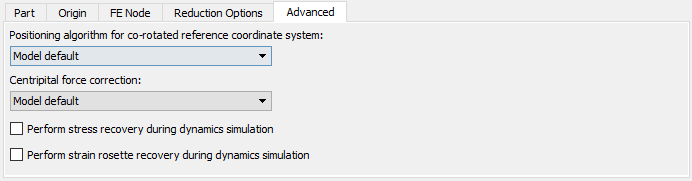
\includegraphics[trim=1 3 90 27,clip,width=0.5\textwidth]
                  {\ReferenceImg/prp/part-5}
\end{wrapfigure}

To activate recovery during simulation, use the appropriate toggles in the
\protect\hyperlink{advanced-tab}{\sl Advanced tab} of the Property Editor panel
for the Part in question (shown at right, see also
\refSection{part-properties}{Part properties}). You may enable one
or both of these toggles to activate such recovery during simulation for
an FE Part, and can also enable them for several parts in a multi-part
model. Enabling strain rosette recovery will, of course, have no effect
unless strain rosette objects have been defined on that FE part.

\Caution{Doing stress recovery during the dynamics simulation is a costly
  operation, so for models with large FE parts, this will increase the total
  simulation time considerably. Therefore, use this feature only if the
  simulation time is not essential.}


\SubSection{Monitoring the most problematic DOFs during time integration}
           {monitoring-the-most-problematic-dofs-during-time-integration}

For complex models, it is not likely that the dynamics simulation will run
smoothly in the first attempt. Some fine tuning and/or model correction will
often be required before a converged solution can be obtained.
To aid the debugging of problematic models, the DOFs that get the largest
solution increments during the non-linear iterations will be listed in the
\File{.res} file when the simulation experiences convergence problems.
Often, the problem can then be identified by studying the elements related
to these DOFs and verifying that their geometry and/or properties are sane.

Fedem will produce those messages when the convergence criteria employed (see
\refSubSection{tolerances-tab}{Tolerances tab}{dynamics-solver-advanced-mode})
increases in two or more consecutive iterations, or the number of iterations is
getting close to the maximum number of iterations specified.
It is then assumed that a convergence problem is encountered, and the specified
number of the worst DOFs will then be output along with local DOF number,
object entity information, and the actual solution increment in that DOF.

Finally, you can specify the Dynamics Solver to abort the simulation
after a certain number of such poor convergence warnings have been issued.

The DOF monitoring is controlled by means of Additional Solver Options
(see \refSection{additional-solver-options}{Additional solver options}).
The following options are available for this purpose
(default value in parentheses):

\begin{tabular}{ m{3.0cm} m{8.0cm} }
{\tt-monitorWorst} & Number of DOFs to monitor on poor convergence (6) \\
{\tt-monitorIter} & Number of iterations to monitor before {\tt-maxit} (2) \\
{\tt-stopOnDivergence} & Number of warnings on possible divergence before the
                         dynamics simulation is aborted (0 = no limit)
\end{tabular}


\SubSection{Starting the analysis}{starting-the-analysis}

Once you have set up the dynamics solver options, you can start the dynamics
simulation by clicking the \textbf{Run!} button available in any of the tabs
of the Dynamics Solver dialog box, discussed above in
\refSection{dynamics-solver-basic-mode}{Dynamics Solver (Basic Mode)} and
\refSection{dynamics-solver-advanced-mode}{Dynamics Solver (Advanced Mode)}.


\SubSection{Handling singularities during the dynamics analysis}
           {handling-singularities-during-the-dynamics-analysis}

The Dynamics Solver has a similar treatment of singular equations during
the solution of linear equation systems, as the FE model Reducer (see
\refSection{handling-singularities-during-the-model-reduction}
           {Handling singularities during the model reduction}).
All singular DOFs will thus be attempted found in one go, letting you fix
them all before a new analysis is attempted. However, in the Dynamics Solver,
neither type of singularities (true zero pivots, or reduced-to-zero pivots) are
permitted. The solver will therefore abort on any occurrence of singularities
after the triangularization is completed.
All singularities found are then listed in the {\sl Output List} and on the
\File{.res} file. They are identified with the internal node number and the
mechanism entity it is associated with (Triad DOF, Joint DOF or component mode
of a Part).


%%%%%%%%%%%%%%%%%%%%%%%%%%%%%%%%%%%%%%%%%%%%%%%%%%%%%%%%%%%%%%%%%%%%%%%%%%%%%%%%
\Section{Stress recovery analysis}{stress-recovery-analysis}

\SubSection{Stress recovery options}{stress-recovery-options}

\IconTextFirst{stressSetup}{
  To specify parameters for the stress analysis,
  click the \textbf{Stress Recovery Setup} button on the \textbf{Solvers}
  tool bar (or from the \textbf{Solve} menu).}

Each time stress recovery is run, the results are added to the existing stress
recovery results. This means you could solve stresses for one time interval
first, and subsequently for another interval, while stresses from both intervals
could be animated in the same animation.
You could also solve stress first, view them, and solve strains later,
making both stress and strain available for post-processing.

This also means that if stress recovery is performed more than once using
identical settings, the same results will be stored multiple times on disk.
It is not checked whether the results you asked for already exist or not.

\noindent
\begin{minipage}{0.45\textwidth}
  \raggedright
  \begin{bulletlist}
  \item
    To specify the time steps at which stress is recovered, a {\sl Start} time,
    {\sl Stop} time and a time {\sl Increment} should be provided.
    However, if the {\sl Use all time steps} option is enabled, stress recovery
    will be performed for all computed time steps between the specified start
    and stop time. The \textbf{Reset} button restores the default
    {\sl Time Interval} values, which are equal to the start and stop times
    of the simulation as specified in the
    \protect\hyperlink{time-tab}{\sl Time tab} of the Dynamics Solver Setup
    dialog box, and 10 times the initial time increment used in the simulation.
  \end{bulletlist}
\end{minipage}%
\hfill\begin{minipage}{0.5\textwidth}
  \begin{picture}(173,235)
    \put(0,0){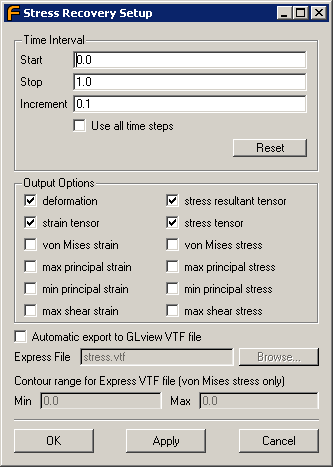
\includegraphics[width=\textwidth]{Figures/Dialogs/6-StressSetup}}
    \put(45,215){\Bullet{1}}
    \put(53,141){\Bullet{2}}
    \put(-8,62){\Bullet{3}}
  \end{picture}
\end{minipage}

\begin{bulletlist}
  \setcounter{enumi}{1}
\item
  You can choose which type of results to recover by activating the appropriate
  {\sl Output Options} toggles. For very large models it is recommended not to
  recover more results than you actually want to animate, as the efficiency of
  the animation process, and the size of the results database files,
  is dependent on the amount of data computed.

\EnumNote{If you choose to recover the stress and/or strain tensors, there is no
  need to also toggle the derived quantities (von Mises, max principal, etc.).
  You may always animate the derived quantities as long you have recovered the
  stress/strain tensors using the {\rm Operation} menu in the Property Editor
  panel of the animation (see
  \refSubSection{contours-tab}{Contours tab}{animation-properties}).}

\item
  You may enable direct export of a GLview Express VTF-file with von Mises
  stress contours and optionally the deformed shape, for further viewing in the
  Ceetron GLview environment (see \href{https://www.ceetron.com}{ceetron.com}).
  You may also need to specify the contour range to be used in the exported
  VTF-file (the maximum and minimum values of the exported von Mises stress
  will be used if no range is specified).
\end{bulletlist}

\Note{The {\rm deformation} toggle in the {\rm Output Options} frame also
  affects the GLview VTF export from the Stress Recovery.
  The deformed shape will thus be exported to the VTF file only when this
  toggle is on. None of the other toggles influence the VTF export.}


\SubSection{Result output control}{result-output-control-1}

As explained above, the Stress Recovery Setup panel may be used to specify the
result types wanted as output from the stress analysis.
There are, however, some additional options for customizing the size and
contents of the results database that may be specified in the Additional Solver
Options dialog box (see
\refSection{additional-solver-options}{Additional solver options}).
Some of these options are discussed below.
The complete list of options to the Stress Recovery solver module is found in
\refSection{stress-options}{Stress recovery options (fedem\_stress)}.

\subsubsection{Output accuracy}

By default the results from a stress recovery analysis are output in single
precision (32-bit real). The output precision may, if so wanted, be set to
double precision (64-bit real) by using the {\tt-double} solver option.


\SubSection{Starting the analysis}{starting-the-analysis-1}

\IconTextFirst{stress}{
  Once you have set up the stress recovery options and performed the dynamics
  simulation, you can start the stress recovery by clicking the
  \textbf{Recover Stress} button on the \textbf{Solvers} tool bar (or from the
  \textbf{Solve} menu). You may also run the stress recovery on a selection
  of parts or on individual element groups, see
  \refSection{part-and-group-wise-solving}{Part- and group-wise solving}.}

\Note{If element calculations fail during stress recovery analysis,
  the recovery continues on the other elements. All failed elements will then
  appear gray in the contour plot after the animation is loaded.}


%%%%%%%%%%%%%%%%%%%%%%%%%%%%%%%%%%%%%%%%%%%%%%%%%%%%%%%%%%%%%%%%%%%%%%%%%%%%%%%%
\Section{Mode shape recovery analysis}{mode-shape-recovery-analysis}

To animate or display detailed mechanism mode shapes, you must first set up and
perform the dynamics analysis and then the mode shape recovery analysis.

\Note{Rigid body mode shapes can also be animated without a mode shape recovery
  analysis (see \refSection{animation-properties}{Animation properties}
  for more information).}


\SubSection{Mode shape options}{mode-shape-options}

\IconTextFirst{modesSetup}{
  To set up the mode shape analysis,
  click the \textbf{Mode Shape Recovery Setup} button on the \textbf{Solvers}
  tool bar (or from the \textbf{Solve} menu).
  The dialog box is opened as shown below. You can then select the modes you
  want to expand and add them to the list of selected modal results.}

\noindent
\begin{minipage}{0.53\textwidth}
  \raggedright
  \begin{bulletlist}
    \setlength\itemsep{1mm}

  \item{\sl Mode:} and {\sl Time:} --
    These are pull-down menus with mode numbers and times at which eigenmodes
    have been (or will be) calculated in the dynamics analysis.

  \item\textbf{Add} button --
    Inserts selected mode shape for the selected time into the results list.

  \item{\sl Mode shapes to recover:} --
    List of selected mode shapes to expand during postprocessing
    (sorted by mode number).

  \item\textbf{Delete} button --
    Removes the selected mode and time from the results list.

  \item You may enable a direct export of \newline a GLview Express VTF-file for
    \newline each recovered mode shape, for further viewing in the
    Ceetron GLview environment (\href{https://www.ceetron.com}{ceetron.com}).
    If a mode shape is to be recovered for more than one time step,
    that shape will be exported to VTF only for the first time step specified.
  \end{bulletlist}
\end{minipage}%
\hfill\begin{minipage}{0.45\textwidth}
  \begin{picture}(155,260)
    \put(0,0){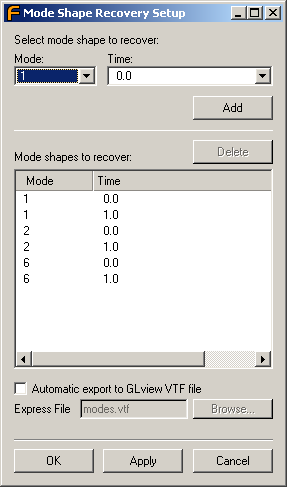
\includegraphics[width=\textwidth]{Figures/Dialogs/6-ModesSetup}}
    \put(43,227){\Bullet{1}}
    \put(88,200){\Bullet{2}}
    \put(35,135){\Bullet{3}}
    \put(88,175){\Bullet{4}}
    \put(-8, 48){\Bullet{5}}
  \end{picture}
\end{minipage}

\Tip{The {\rm Mode:} and {\rm Time:} pull-down menus both have an {\rm (All)}
  entry in the bottom to facilitate easy selection of all entries in the list.
  This is useful if you want to recover all mode shapes and/or the selected
  mode shape for all time steps at which it has been computed.}

\clearpage
\Note{The expanded mode shapes for one part are stored in a single \File{.frs}
  file provided all modes are expanded for the same set of time steps.
  However, if only one mode is expanded for a different set of time steps than
  the other modes, one \File{.frs} file is created for each expanded mode.
  Therefore, if you are expanding a large amount of modes, it is advised to
  select the same time steps for all modes in order to limit the number of files
  in the results database as this might impact the post-processing performance.}


\SubSection{Starting the analysis}{starting-the-analysis-2}

\IconTextFirst{modes}{
  Once you have set up the mode shape recovery options and performed the
  dynamics simulation, you can post process the modes at the selected times
  by clicking the \textbf{Recover Mode Shapes} button on the \textbf{Solvers}
  tool bar (or from the \textbf{Solve} menu).}

When Fedem has postprocessed all the selected modes, you can animate the
mode shapes (see \refSection{animations}{Animations} for more information).


%%%%%%%%%%%%%%%%%%%%%%%%%%%%%%%%%%%%%%%%%%%%%%%%%%%%%%%%%%%%%%%%%%%%%%%%%%%%%%%%
\Section{Strain rosette analysis}{strain-rosette-analysis-1}

The strain rosette analysis recovers the stresses and strains on the virtual
strain rosettes defined in your model.
See \refSection{strain-rosettes}{Strain rosettes} on how to create and edit
virtual strain rosettes. The output is similar to the output from real strain
gages in addition to standard strain and stress quantities like Von Mises,
principal stresses/strains, and angle of max/min. principals.

\clearpage


\SubSection{Strain rosette options}{strain-rosette-options}

\IconTextFirst{gageSetup}{
  To specify strain rosette analysis parameters,
  click the \textbf{Strain Rosette Recovery Setup} button on the
  \textbf{Solvers} tool bar (or in the \textbf{Solve} menu).}

\noindent
\begin{minipage}{0.52\textwidth}
  \raggedright
  \begin{bulletlist}
  \item
    You can specify the {\sl Start} and {\sl Stop Time} for strain rosette
    recovery and the {\sl Time Increment} at which to recover the rosettes.
    If the {\sl Use all time steps} option is enabled, rosette recovery will be
    performed for all computed time steps between the specified start and stop
    time. The \textbf{Reset} button restores the default {\sl Time Interval}
    values, which are equal to the start and stop times of the simulation, as
    specified in the Dynamics Solver Setup, and using all time steps in between.
  \end{bulletlist}
\end{minipage}%
\hfill\begin{minipage}{0.45\textwidth}
  \begin{picture}(155,164)
    \put(0,0){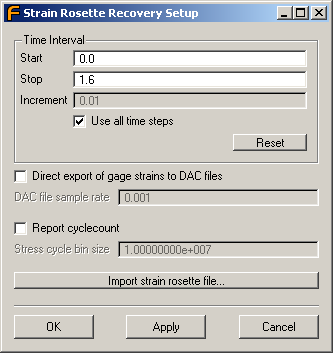
\includegraphics[width=\textwidth]{Figures/Dialogs/6-GageSetup}}
    \put(-8,135){\Bullet{1}}
    \put(-8,77){\Bullet{2}}
    \put(-8,52){\Bullet{3}}
    \put(-8,29){\Bullet{4}}
  \end{picture}
\end{minipage}

\begin{bulletlist}
  \setcounter{enumi}{1}
\item You may enable
  a direct export of gage strains to DAC files with a specified sample rate.
\item You may enable
  a stress cycle count with a specified bin size. The results are written to
  the file \File{fedem\_gage.res} when running the strain rosette recovery.
  The computed damage will also be reported to this file for all
  strain rosettes when this option is enabled.
\item Strain rosette definitions can be imported from a file by pressing this
  button. The strain rosettes defined will then be read into Fedem, and virtual
  strain rosettes will be created automatically based on the definitions. See
  \refSection{strain-rosette-definition-file-format}
             {Strain rosette definition file format}
  for the format of this file.
\end{bulletlist}


\SubSection{Starting the analysis}{starting-the-analysis-3}

\IconTextFirst{gage}{
  Once you have set up the strain rosette recovery options and performed the
  dynamics simulation, you can start the strain rosette recovery by clicking the
  \textbf{Recover Strain Rosettes} button on the \textbf{Solvers} tool bar
  (or from the \textbf{Solve} menu).}


\SubSection{Result output}{result-output}

Results for all strain rosettes on a part are output to the binary \File{.frs}
file named \File{\textless partname\textgreater\_\#.frs}.
The \File{.frs} file allows the post-processing of strain rosette recovery
results through graphs.

In addition to the default stress and strain results, you may also output the
nodal deformations in the strain rosettes to the \File{.frs} file, by specifying
{\tt-deformation} as an additional option to the Strain Rosette Recovery
(see \refSection{additional-solver-options}{Additional solver options}).

If enabled, a file named \File{rosette{\sl ID}\_gage{\sl n}.dac} is written
for each strain gage, containing the strain of leg {\sl n} in strain rosette
{\sl ID}. This file is output in the nCode DAC format.

It is also possible to output the strain rosette result directly to ASCII files.
By specifying {\tt-writeAsciiFiles} as an additional option to the
Strain Rosette Recovery, you will get a file named
\File{rosette{\sl ID}.asc} for each strain rosette defined.
A summary of contents for this ASCII file is given below.

All of the above mentioned files are created in separate directories for each
part, which then are placed in the sub-directory
\File{timehist\_gage\_rcy\_\#\#\#\#/} in the result file hierarchy
(see \refSection{rdb-directory-structure}{RDB directory structure}).

\subsubsection{ASCII output file format}

The \File{rosette{\sl ID}.asc} file contains a heading and a data section.
(See file cutout below.) The heading summarizes the strain rosette definition,
the data section lists all measurements made.

\begin{figure}[!h]
  \center
  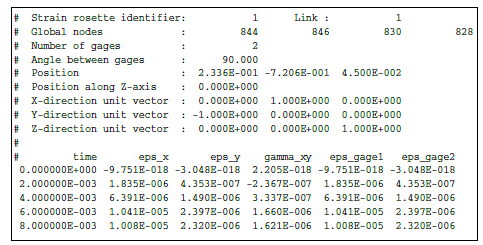
\includegraphics[width=0.9\textwidth]{Figures/6-StrainRosette-TextOutput}
\end{figure}

\clearpage
Note that this cutout is an edited version not showing the entire file contents.
Detailed information on the full contents of the data section is listed
in the table below. All angles are output in degrees.

\begin{tabular}{| m{19mm} | m{85mm} |}
  \hline
  Data output    &  Description of output \\
  \hline\hline
  {\sl Time}     & Time \\
  $\epsilon_x$   & Strain XX in rosette coordinate system \\
  $\epsilon_y$   & Strain YY in rosette coordinate system \\
  $\gamma_{xy}$   & Shear strain XY in rosette coordinate system \\
  $\epsilon_1$   & First principal strain \\
  $\epsilon_2$   & Second principal strain \\
  $\gamma_{max}$  & Max shear strain \\
  $\alpha_1$     & Angle from rosette X-axis to direction of principle strain \\
  $\alpha_\gamma$ & Angle from rosette X-axis to direction of max shear \\
  $\sigma_x$     & Stress XX in rosette coordinate system \\
  $\sigma_y$     & Stress YY in rosette coordinate system \\
  $\tau_{xy}$     & Shear stress XY in rosette coordinate system \\
  {\sl von Mises} & von Mises stress \\
  $\sigma_1$      & First principal stress \\
  $\sigma_2$      & Second principal stress \\
  $\tau_{max}$     & Max shear stress \\
  $\epsilon_{gage1}$ & Strain in leg 1 \\
  $\epsilon_{gage2}$ & Strain in leg 2 \\
  $\epsilon_{gage3}$ & Strain in leg 3 \\
  \hline
\end{tabular}

\subsubsection{File buffering and flush frequency}

The output to the \File{.frs} file may be controlled using the additional option
{\tt-flushinc}, which works in the same manner as with the Dynamics Solver
(see \refSection{result-output-control}{Result output control}).
However, the default value is here -1.0, i.e., the file is flushed to disk
when the internal fixed-size file buffer is filled.
Note that this option only affects the \File{.frs} file output.

The DAC and ASCII file output is not affected.

\clearpage


\SubSection{Strain rosette definition file format}
           {strain-rosette-definition-file-format}

It is possible to define strain rosettes in an ASCII input file, as
shown in the example below, and read them into Fedem.

\begin{figure}[!h]
  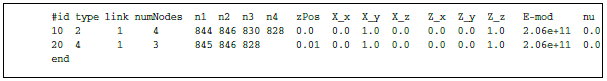
\includegraphics[width=\textwidth]{Figures/6_StrainRosette_file_format}
\end{figure}

Each line defines a strain rosette, where the following data must be given:
%
\begin{namelist}{\bf type:}
\item[\sl\textbf{id:}]
  The id number is used for naming purposes of the result files.
  The above example defines two strain rosettes,
  with identifiers 10 and 20 respectively.

\item[\sl\textbf{type:}]
  According to the figure below, rosette 10 is of type 2, i.e., a two gages
  with 90 degrees between the gages, whereas rosette 20 is of type 3,
  three gages with 60 degrees between the gages.

  \hspace*{-0.33\textwidth}
  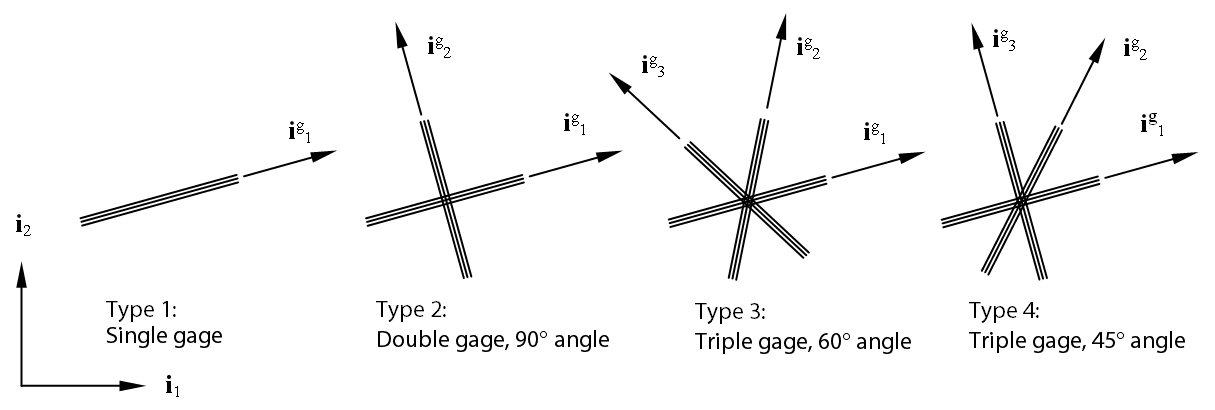
\includegraphics[width=1.2\textwidth]{Figures/6-StrainGages}

\item[\sl\textbf{link:}]
  The superelement (part) number that the present rosette is attached to.

\item[\sl\textbf{numNodes n1 n2 n3 (n4):}]
  Number of nodes for the element followed by node numbers that define the
  element topology. Permissible values for numNodes are 3 and 4,
  giving CST triangle and bi-linear quad element respectively.
  The nodal numbers must be given in a circular fashion around the element,
  where both clockwise and counterclockwise sequences are permitted.
  The node numbers will possibly be reversed internally so that the element
  Z-axis points in the user defined direction.

\item[\sl\textbf{zPos:}]
  Defines the location of the rosette along the $Z$-axis.
  If the user wants the strains measured at the top of a plate, the number at
  the Z-pos column should be $h/2$ where $h$ is the plate thickness.
  A value of $-h/2$ will give the strains at the bottom of the plate.

\item[\sl\textbf{X\_x X\_y X\_z:}]
  These three numbers define a vector, which is used to define the local
  $X$-direction for the rosette coordinate system. The vector is given in
  the part coordinate system. The vector does not need to be given as a unit
  vector, nor does the vector need to lie exactly in the element plane.
  The $X$-direction used for computations is obtained through a projection
  of the user-defined vector onto the element plane.

\item[\sl\textbf{Z\_x Z\_y Z\_z:}]
  These three numbers represent a vector, which is used for defining
  the positive Z direction of the rosette coordinate system.
  The vector defined by the user does not need to be exactly perpendicular
  to the element plane. As long as the vector has a component pointing
  out from the element plane, the $Z$-direction for the rosette coordinate
  system will be correctly defined.
  The rosette $Y$-direction is implicitly defined through the $X$-
  and $Z$-directions.

\item[\sl\textbf{E-mod nu:}] Young's modulus (E-mod) and Poisson's ratio (nu)
  are used for computing the stress state at the rosette location.
\end{namelist}


%%%%%%%%%%%%%%%%%%%%%%%%%%%%%%%%%%%%%%%%%%%%%%%%%%%%%%%%%%%%%%%%%%%%%%%%%%%%%%%%
\Section{Strain coat analysis}{strain-coat-analysis-1}

This analysis recovers the stresses and strains on all strain coat elements in
the model, and calculates a summary of the recovered results as it processes.
The output from the strain coat analysis is a result database (\File{.frs})
file for each part containing the maximums of certain stress/strain quantities
over the time interval considered.
Optionally, you may also perform a rainflow and fatigue analysis based on the
computed stress or strain histories during the strain coat recovery.
The result files from the strain coat analysis are created in separate
directories for each part below the \File{summary\_rcy\_\#\#\#\#/} directory in
the result file hierarchy
(see \refSection{rdb-directory-structure}{RDB directory structure}).

\clearpage


\SubSection{Generating strain coat}{generating-strain-coat}

\begin{wrapfigure}[17]{r}{0.35\textwidth}
  \vspace{-5mm}
  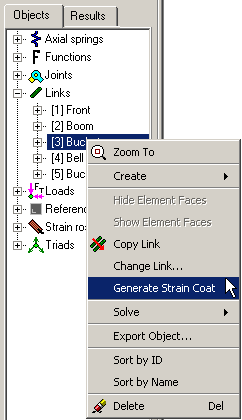
\includegraphics[width=0.35\textwidth]{Figures/6-GenerateStraincoat}
\end{wrapfigure}

Before you run the strain coat analysis, you must generate strain coat elements
for the parts or element groups in question. This is done by right-clicking the
parts or groups in the {\sl Objects} list of the Model Manager panel
and selecting \textbf{Generate Strain Coat} from the menu.
Again, multi-selection is possible.

One strain coat element is created for each non-interior face of the finite
elements in the current selection. If a strain coat element already exist for a
given face, a new strain coat element is not created.
Therefore, repeating the \textbf{Generate Strain Coat} command for
the same selection has no effect.

When creating strain coat elements by selecting an element group the new
strain coat elements are automatically added to that group.

If a part is selected, the created strain coat elements are only added to the
implicit element groups which the parent finite element belongs to, not to any
explicit element groups that the parent element might be a member of.
Refer to \refSection{element-groups}{Element groups}
to learn about implicit and explicit groups.

\Note{The strain coat elements will appear in the \File{.ftl} file
  in the FE model repository when the model is saved.}


\SubSection{Strain coat analysis options}{strain-coat-analysis-options}

\IconTextFirst{fpp}{
  To specify parameters for the strain coat analysis,
  click the \textbf{Strain Coat Recovery Summary Setup} button on the
  \textbf{Solvers} tool bar (or from the \textbf{Solve} menu).}

\clearpage
\noindent
\begin{minipage}{0.52\textwidth}
  \raggedright
  \begin{bulletlist}
    \setlength\itemsep{1mm}
  \item
    You can specify the {\sl Start} and {\sl Stop} time for strain coat recovery
    summary and the time {\sl Increment} to be used.
    However, if the {\sl Use all time steps} option is enabled, all computed
    time steps between the specified start and stop time will be considered.
    The \textbf{Reset} button restores the default {\sl Time Interval} values
    which are equal to the start and stop times of the simulation as specified
    in the Dynamics Solver dialog box, and to use all time steps in between.
  \item
    You may limit the number of elements to be processed concurrently by
    adjusting this value. Especially for large parts and long time series
    this might be necessary due to higher memory requirements.
\end{bulletlist}
\end{minipage}%
\hfill\begin{minipage}{0.45\textwidth}
  \begin{picture}(155,252)
    \put(0,0){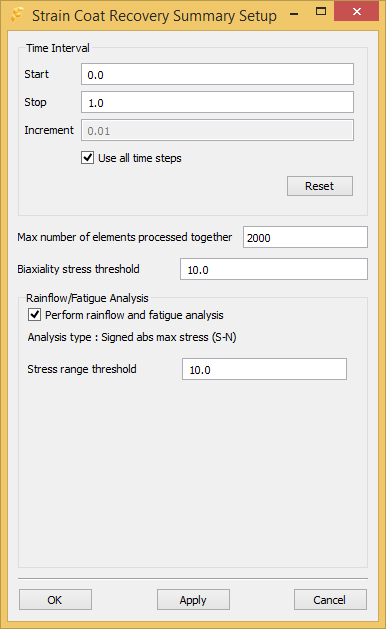
\includegraphics[width=\textwidth]{Figures/Dialogs/6-FppSetup}}
    \put(-7,226){\Bullet{1}}
    \put(-7,152){\Bullet{2}}
    \put(-7,138){\Bullet{3}}
    \put(-7,121){\Bullet{4}}
    \put(-7,110){\Bullet{5}}
    \put(-7,99){\Bullet{6}}
  \end{picture}
\end{minipage}

\begin{bulletlist}
  \setcounter{enumi}{2}
\item
  You may set a gate value for the {\sl Biaxiality} calculation.
  That is, the mean biaxiality will be computed only for elements whose max
  principal stress is larger than the specified threshold value.
\item
  You may toggle On/Off rainflow and fatigue analysis. The remaining options in
  this dialog box are sensitive only when this toggle is {\sl On}.
\item
  The Analysis type is always {\sl Signed abs max stress (S-N)}.
\item{\sl Stress/Strain range threshold}:
  You may set a gate value for the {\sl Peak valley extraction}.
  That is, only the stress/strain ranges with magnitude higher than this value
  will be included in the peak valley extraction.
\end{bulletlist}

To perform rainflow and fatigue analysis during the strain coat recovery,
you also need to assign an S-N curve to base the damage calculation on,
for each element group you want to consider in the fatigue analysis.
This is performed in the Property Editor panel for the element groups,
see \refSection{element-group-properties}{Element group properties}.


\SubSection{Starting the analysis}{starting-the-analysis-4}

\IconTextFirst{fppSetup}{
  Once you have set up the strain coat recovery summary options and performed
  the dynamics simulation, you can start the strain coat recovery by clicking
  the \textbf{Recover Strain Coat Summary} button on the \textbf{Solvers}
  tool bar (or from the \textbf{Solve} menu).
  The Strain Coat Recovery is then performed on each part in the model
  containing strain coat elements.
  Parts without strain coat elements are automatically omitted.}


\SubSection{Strain coat recovery on element groups or individual parts}
           {strain-coat-recovery-on-element-groups-or-individual-parts}

A strain coat recovery can also be performed on defined element groups
or a selection of parts.
See \refSection{part-and-group-wise-solving}{Part- and group-wise solving}
to learn how such a process is started.
In this case, strain coat elements are created automatically for the
selected part(s) or element group(s), before the recovery process is started.
It is therefore no need to do this manually, as explained in
\refSection{generating-strain-coat}{Generating strain coat}, in this case.


%%%%%%%%%%%%%%%%%%%%%%%%%%%%%%%%%%%%%%%%%%%%%%%%%%%%%%%%%%%%%%%%%%%%%%%%%%%%%%%%
\Section{Direct linear analysis of FE Parts}{direct-linear-analysis-of-fe-parts}

Instead of doing a full dynamic simulation with subsequent stress recovery,
it is also possible to perform a direct linear FE analysis on individual parts.
This is handy if you only want to asses the static properties of a FE model
before using it in a larger mechanism simulation.

A direct linear FE analysis of a Part is performed while keeping all Triads
defined on the part fixed. Alternatively (or in addition), more detailed
boundary conditions on individual nodal points in the part may be defined in
the FE model file (see \refSection{using-fe-models}{Using FE models}).
Any loads defined in that file will also be accounted for,
in addition to gravity loads (if a gravitation vector is defined,
see \refSection{gravitation}{Gravitation}).
All other mechanism objects (Joints, springs, etc.), if any, will be ignored.

Therefore, performing a linear analysis on an assembly of FE parts will be the
same result as performing the analysis on each part separately.


\SubSection{Starting a direct linear analysis}
           {starting-a-direct-linear-analysis}

A direct linear analysis can only be started as a Part-wise solve process, see
\refSection{part-and-group-wise-solving}{Part- and group-wise solving}, since
no coupling will exist between multiple parts in the model during the analysis.

\begin{wrapfigure}[16]{r}{0.5\textwidth}
  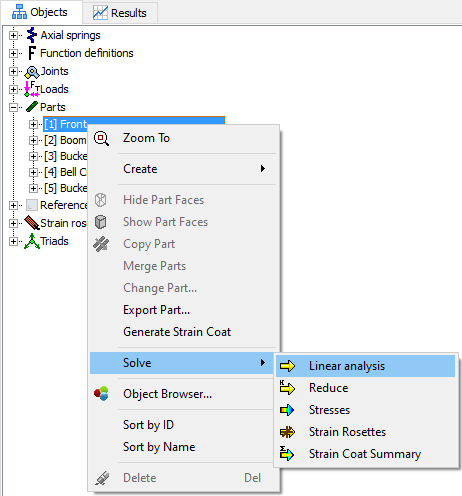
\includegraphics[width=0.5\textwidth]{Figures/6-SolveLinearAnalysis.png}
\end{wrapfigure}

Start the process by right-clicking on the part (or parts) in the {\sl Objects}
list of the Model Manager panel, and choose \textbf{Solve} and then
\textbf{Linear Analysis} from the menu (as shown to the right).

The results of a linear analysis is only the displacement field, which then can
be viewed in an Animation object. However, it is possible to also perform
a Part-wise stress recovery on the same part afterwards, to compute stresses
based on the computed displacement field. This stress recovery will perform the
same simulation as the normal stress recovery process described in
\refSection{stress-recovery-analysis}{Stress recovery analysis},
except that the recovered displacements are read from a file instead of being
computed from the system response of the dynamics simulation.

\Note{The result files from a Linear analysis is stored in the same location
  as the results files from a stress recovery of that part.}


%%%%%%%%%%%%%%%%%%%%%%%%%%%%%%%%%%%%%%%%%%%%%%%%%%%%%%%%%%%%%%%%%%%%%%%%%%%%%%%%
\Section{Interaction during processing}{interaction-during-processing}

\SubSection{Simultaneous viewing and processing}
           {simultaneous-viewing-and-processing}

If you already have set up graphs and animations (see
\refChapter{postprocessing-results}{Postprocessing Results}),
they can be viewed during the dynamics analysis.
Your graphs and 3D views can be dynamically updated to show the results from the
mechanism as they are computed.

\subsubsection{Graphs}

If graph views are displayed (see \refSection{showing-a-graph}{Showing a graph})
during the dynamics simulation, each curve is continuously updated with values
from the solution, reflecting the progress of the dynamics analysis.

\Tip{A graph showing the number of iterations for each time step gives a
  good indication of both the progress of the simulation, and how quickly
  each time step converges to the specified tolerance.}

\subsubsection{Animations}

If a 3D animation is loaded (see
\refSubSection{loading-animations}{Loading animations}{managing-animations})
the dynamics simulation, the 3D view of the model is continuously updated with
the rigid body motion of the part, reflecting the simulation results. The model
can also be examined (rotated, zoomed, and so on) during the animation.

\Tip{The rigid body animation is an effective and intuitive way to observe
  the progress of the simulation. When the rigid body animation is displayed,
  a progress bar also appears in the upper-right corner of the Modeler view.}

\Tip{A rigid body animation may be started automatically when the dynamics
  solver starts by enabling a toggle in the Dynamics Solver Setup (see
  \refSubSection{output-tab}{Output tab}{dynamics-solver-advanced-mode}).}

\Tip{Animations can be loaded and closed at any time during the simulation.}

\Caution{With large models and long simulations, the simultaneous visualization
  and simulation features may use a large amount of system resources.}


\SubSection{Stop processing}{stop-processing}

\IconTextFirst{stop}{
  Solution processes can be stopped at any time by pressing the
  \textbf{Stop All Solvers} button on the \textbf{Solvers} tool bar
  (or in the \textbf{Solve} menu).}

\Note{All results created before the \textbf{Stop} button is pressed are stored
  and can be evaluated in the normal manner.}


%%%%%%%%%%%%%%%%%%%%%%%%%%%%%%%%%%%%%%%%%%%%%%%%%%%%%%%%%%%%%%%%%%%%%%%%%%%%%%%%
\Section{Deleting results}{deleting-results}

\IconTextFirst{eraseAllRes}{
  To delete result files from the dynamics simulation and recovery operations
  (stress recovery, modes recovery, strain rosette recovery and strain coat
  recovery), click the \textbf{Delete Results} button on the \textbf{Solvers}
  tool bar (or in the \textbf{Result} menu).}

\Note{Result files are not deleted until you save or close the model,
  and files from model reductions are never deleted.}

\Caution{If you use the \textbf{Save As...} command to save a model to a
  different location, result files from previous solutions are not
  copied to the new location.
  Only result files and reduced parts from the current analysis are copied.
  (Applicable only if the {\sl Discard results} and {\sl Discard reduced parts}
  toggles are not set.}


\SubSection{Deleting specific results}{deleting-specific-results}

Results from specific recovery processes can be deleted independently.
This is useful for reclaiming disk space or changing the results set available
for the subsequent post-processing operations.

\def\DeleteRecoveryResults#1#2#3{
  \IconText{#1}{The #2 recovery results can be deleted by clicking the
  \textbf{Delete #3 results} button on in the \textbf{Results} menu.}}

\DeleteRecoveryResults{deleteStressResults}
                      {stress}{Stress Recovery}

\DeleteRecoveryResults{deleteModesResults}
                      {mode shape}{Mode Shape Recovery}

\DeleteRecoveryResults{deleteRosetteResults}
                      {strain rosette}{Strain Rosette Recovery}

\DeleteRecoveryResults{deleteStrainCoat}
                      {strain coat}{Strain Coat Recovery Summary}

\Note{The results files are deleted immediately when performing these actions.}


%%%%%%%%%%%%%%%%%%%%%%%%%%%%%%%%%%%%%%%%%%%%%%%%%%%%%%%%%%%%%%%%%%%%%%%%%%%%%%%%
\Section{Automated curve export from multiple result database files}
        {automated-curve-export-from-multiple-result-database-files}

If you need to export curve data from several result database files into
a single output file (e.g., if you want curves from one or more Strain Rosette
analyses exported to a single RPC-file or a multi-columns ASCII file),
that can be done by executing the Fedem Curve Export Utility module after the
necessary solver tasks have been completed.

The curve export utility can only be invoked as a separate command from
a terminal window or command prompt.
Start the curve export by issuing the following command:

\texttt{
  fedem\_graphexp -frsFile (fnames) -modelFile (mname) \textbackslash
  \newline\hspace*{32mm}
  -curvePlotFile (cname) [\textless options\textgreater]}

\noindent
where {\tt(fnames)} is a list of one or more \File{.frs} files on the form
\File{\textless file1,file2,...\textgreater}, {\tt(mname)} is the Fedem model
file (\File{.fmm}) in which the curves to be exported are defined, and
{\tt(cname)} is the name of the output file where the curve data is exported.
The module also have some other options to facilitate the export process
(see \refSection{curve-export-options}{Curve export options (fedem\_graphexp)}
for a complete list of all options).


%%%%%%%%%%%%%%%%%%%%%%%%%%%%%%%%%%%%%%%%%%%%%%%%%%%%%%%%%%%%%%%%%%%%%%%%%%%%%%%%
\Section{Batch execution of solver processes}
        {batch-execution-of-solver-processes}

If you need to run several versions of a model, it is often most efficient to
edit the model file directly in an editor, or by means of scripting, and then
run the solver processes in batch mode from a terminal window or the
command-line prompt. To facilitate such batch executions, a set of command-line
options is provided, that run Fedem in a non-graphics and non-interactive mode
(see \refSection{fedem-gui-options}{Fedem GUI options} for the complete list
of command-line options for the Fedem UI).


\SubSection{Batch solving trough the User Interface}
           {batch-solving-trough-the-user-interface}

Start the Fedem UI from the command-line prompt with the following command:

\texttt{fedem -f (mname) -solve (sname)}

\noindent
where {\tt(mname)} is the Fedem model file and {\tt(sname)} is one of the
keywords {\sl reducer}, {\sl dynamics}, {\sl stress}, {\sl modes},
{\sl straingage}, {\sl straincoat}, {\sl events} or {\sl all}.
This will read the specified model file, and immediately launch the specified
solver process(es), and then save the model file and the obtained results before
the command exits.
Thus, this has the same effect as (but is normally faster) the following steps:

\begin{enumerate}
\item Start the Fedem UI interactively in the normal manner
\item Open the desired model file
\item Launch the desired solver process from the \textbf{Solvers} tool bar
\item Exit Fedem with saving of model file
\end{enumerate}

In the same way as when running from the \textbf{Solver} tool bar (or from the
\textbf{Solve} menu), it is checked that all parts are reduced and up to date,
and that dynamics results exist, before a recovery process is started.
And if needed, the necessary pre-requisite solver tasks are executed first.
Thus, to simply run all recovery types on all parts for a given model file,
you can just use the option {\tt -solve all} and all required solver tasks
will be executed sequentially without user interaction.


\SubSection{Preparing for batch solving on remote computers}
           {preparing-for-batch-solving-on-remote-computers}

Sometimes it is desirable to execute solver processes directly on
another computer than the Fedem UI is run on, and which have a separate
file system. It is then necessary to create the needed RDB directory
structure locally, populated with all the required solver input files,
and then manually transfer it to the remote computer for batch execution
(see \refSection{rdb-directory-structure}{RDB directory structure}
for details on the RDB structure).

When finished, the whole directory structure can then be copied back
onto the local computer for further post-processing in the Fedem UI.

\IconText{prepareForBatch}{
  To create a complete RDB structure with input files for all the
  Fedem solver processes, select \textbf{Prepare for batch execution}
  from the \textbf{Solve} menu.}

The RDB structure required for a certain solver process can also be
created by issuing the following command from a terminal window:

\File{fedem -f (mname) -prepareBatch (sname)}
%
\vskip\parskip\noindent
where the meaning of \File{(mname)} and \File{(sname)} is as explained in
\refSection{batch-solving-trough-the-user-interface}
           {Batch solving trough the User Interface}.
Thus, the effect of this command is exactly the same as with the {\tt-solve}
option, except that the solver processes themselves are not executed.
Specifying {\sl all} for {\tt(sname)} with this command is equivalent to using
the \textbf{Prepare for batch execution} entry in the \textbf{Solve} menu.
When the command exits you have the necessary RDB directory structure,
which can be transferred to a remote computer for batch execution.


\SubSection{How to read error messages from the solvers}
           {how-to-read-error-messages-from-the-solvers}

When a solver process fails to complete, or any abnormality occur during the
simulation, messages explaining the problem are written to the {\sl Output List}
during the process execution.
These messages are prefixed either by {\sl Error:}, {\sl Warning:}
or {\sl Note:} signifying something about their severity, as follows:

\begin{namelist}{\textbf{Warning:}}
\item[\textbf{Error:}]
  A problem has occurred that makes it impossible or undesirable to continue
  the simulation. The simulation is aborted in a controlled manner.

\item[\textbf{Warning:}]
  A problem has occurred that may affect the simulation results,
  although the simulation itself continues. However, one should be more critical
  to obtained results when warnings occur, and consider changing the model.

\item[\textbf{Note:}]
  The event causing this kind of message is usually of no significance for the
  results. The message informs the user that an action has been made to perform
  a specific task, etc.
\end{namelist}

When a simulation process aborts with {\sl Error:}-messages, you will also see
the message {\sl See fedem}\_(solver){\sl .res for further details.}
That means that sometimes (but not always) there are further error messages
on the \File{.res} file explaining the problem.
Note, however, that these additional messages are often of a low-level
character and harder to understand for the average user.
The main rule is that messages written to the {\sl Output List} view should be
sufficient to understand the scope of the problem.

\Tip{You can view the \File{.res} file from a simulation process
  using the Result file browser, see
  \refSection{the-result-file-browser-dialog}{The Result File Browser dialog}.}

A solver error will often create several messages on the \File{.res} file,
all related to the same problem/incident. This typically happens if an exception
or error occurs deep inside a program module and from there writes an error
message on what is wrong (basing the message on the knowledge available to that
module). As the program trace-back unfolds, more messages on the same problem
may be produced, providing more information on the problem as it becomes
available. These higher-level messages can be more user friendly due to more
available information. Some messages on the lowest level will have meaning for
the program developers only. It is, however, often necessary to have both the
higher level and the lower level messages to get the full insight.

So, to understand the problem quickly, it is therefore helpful to read these
messages in reverse order, starting with the last message (the highest level)
and ending with the first one (lowest level). Sometimes you may ignore the
lowest level messages (those output to the \File{.res} file only)
and still see what caused the problem.


%%%%%%%%%%%%%%%%%%%%%%%%%%%%%%%%%%%%%%%%%%%%%%%%%%%%%%%%%%%%%%%%%%%%%%%%%%%%%%%%
\Section{Using simulation events}{using-simulation-events}

In many analysis projects using Fedem, the task is to investigate the response
on a given structural model, or a set of almost identical models,
for a large set of load cases, or events. To facilitate such projects,
Fedem has introduced the concept of {\sl Simulation events}.

A simulation event is a small permutation of the structural model, where only a
few model parameters, (such as a load amplitude, a spring stiffness, a cross
section area, etc.) have different values. Each event is then solved and
assigned a separate result database, all within the same model.
That way it is efficient to continue working on the model without needing to
duplicate the input data more than necessary, when setting up the different
load cases. The simulation events can both be run individually, one-by-one,
or all together in a large batch execution.


\SubSection{Setting up simulation events}{setting-up-simulation-events}

When you have established the main part of the model, or at least that part that
is subjected to variation in the multiple load case study, you can create the
simulation events. That is done through the import of an event definition file,
by selecting \textbf{Import events...} from the \textbf{Mechanism} menu.

\subsubsection{Event definition file}

The event definition file is an ASCII file that can be created in a text editor.
It contains a tabular definition of the simulation events, where keywords
representing the model quantities subjected to variation, are the same as those
found in the Fedem model file (\File{.fmm}).
A sample event definition file is shown below.

\begin{figure}[!h]
  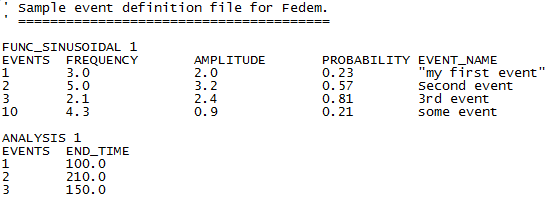
\includegraphics[width=\textwidth]{Figures/6-EventDefSample}
\end{figure}

\noindent
All lines starting with non-letter characters are regarded as comments.

\begin{itemize}
\item
  The first non-comment line should specify the object for which one or more
  model quantities are to be varied in the event.
  The object is specified via its model file keyword followed by the user ID.
\item
  Then comes the event specification for this object:
  \begin{itemize}
  \item[--]
    The first line must begin with the keyword EVENTS, and then the names of the
    data fields to be varied for this object are listed (FREQUENCY and AMPLITUDE
    in the sample above).
  \item[--]
    Then one line for each event follows with the actual data.
    \end{itemize}
\item
  The first column becomes the user ID of the generated event objects.
\item
  The event probability may be added in a separate column (the fourth column in
  the sample above) for each event. The probability is used in Fatigue analysis
  as a weighting factor, when calculating the expected life time of a component
  based on all the simulated load cases.
\item
  The events may optionally be named (the fifth column in the sample above).
  The event name becomes the Description of the event, visible in the
  {\sl Objects} list of the Model Manager panel.
\item
  If more than one object is subject to variation, a new, similar table may
  follow with the EVENTS numbers repeated.
\end{itemize}

\Tip{Use the Object browser (see \refSection{object-browser}{Object Browser})
  to see the model file keyword and associated data field names pertaining to
  the different objects types.}


\SubSection{Event definition dialog}{event-definition-dialog}

Once you have imported an event definition file, you can view the definitions of
the imported events by selecting \textbf{Event Definitions ...} from the
\textbf{Mechanism} menu. The Event Definitions dialog box (shown below) is then
opened. It contains a tabular descriptions of the simulation events,
with a single row for each event and the data fields to be modified as columns.
The column headings resembles the event definitions file.

\begin{figure}[!h]
  \center
  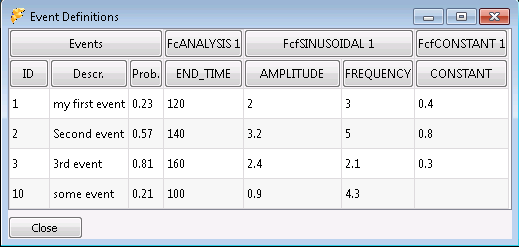
\includegraphics[width=0.8\textwidth]{Figures/Dialogs/6-EventDef}
\end{figure}

Use this dialog box to verify that your events have been correctly defined
before the simulations are started, or to review the parameters for the
different events without having to look in the event definition file itself.


\SubSection{Simulation event properties}{simulation-event-properties}

The Property Editor panel for the simulation events is shown below.
Only the {\sl Description} and {\sl Event probability} fields can be edited
in this panel after the event has been created.

\begin{wrapfigure}[6]{r}{0.5\textwidth}
  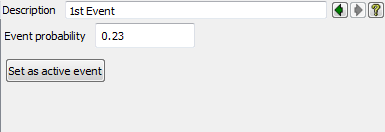
\includegraphics[width=0.5\textwidth]{Figures/6-SimulationEventProperty1}
\end{wrapfigure}

By pressing the \textbf{Set as active event} button, the mechanism elements
are modified according to the definition of the selected event.
Subsequent solve commands and post-processing (graph plotting and
animations) will then be associated with this event.

\begin{wrapfigure}[6]{r}{0.5\textwidth}
  \vspace{-4mm}
  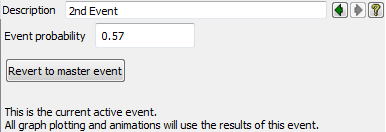
\includegraphics[width=0.5\textwidth]{Figures/6-SimulationEventProperty2}
\end{wrapfigure}

The \textbf{Revert to master event} button will restore the model to how it was
without the modifications imposed by the current active event.
Solving and post-processing will then be associated with the {\sl master} event.


\SubSection{Solving multiple events and result organisation}
           {solving-multiple-events-and-result-organisation}

Each event can be solved and post-processed individually by using the
\textbf{Set as active event} button in the Property Editor panel,
as described above in
\refSection{simulation-event-properties}{Simulation event properties}.

\vskip\parskip
\IconText{solveEvents}{
  It is also possible to start all events simultaneously.
  This is done by clicking the \textbf{Solve all Events} button,
  or selecting \textbf{Solve Events} from the \textbf{Solve} menu.
  Each event is then activated in turn and solved, sequentially or in parallel,
  depending on the {\sl Max concurrent processes} setting in
  the Additional Solver Options dialog box,
  see \refSection{additional-solver-options}{Additional solver options}.}

\begin{wrapfigure}[6]{r}{0.4\textwidth}
  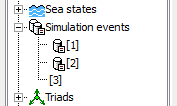
\includegraphics[width=0.32\textwidth]{Figures/6-SimulationEvents}
\end{wrapfigure}

As the different events are being solved, they get an icon in the {\sl Objects}
list of the Model Manager panel indicating that they have simulation results,
as shown to the right. Here, the two first events already have got some results
whereas the third event is still without results.

\Note{The change of event icon is the only user feedback during simulation of
  multiple events, in addition to any messages in the {\rm Output List} view.
  It is not possible to simultaneously plot results or view animations
  while the events are being solved.
  Only when event currently defined as the active event is being solved,
  one can simultaneously view the progress of that one.}

\Note{The \textbf{Solve Events} command works as the \textbf{Solve All}
  command (see \refSection{solvers-tool-bar}{Solvers tool bar}) on the
  individual events. Therefore, stress recovery, mode shape recovery, etc.,
  will also be performed, if enabled, on each event. If that is not desired,
  you have to deactivate those analyses first by setting their start times
  larger than the stop time in the appropriate setup dialog boxes.}

\subsubsection{Managing simulation event results}

The structure of the results database on disk in general is described in
\refSection{rdb-directory-structure}{RDB directory structure}.
However, when simulation events are being used, we get one extra directory
level. Directly under the \File{[modelname]\_RDB} directory, you will have
directories named \File{event\_\#\#\#} and under each of them the normal
response directories \File{response\_\#\#\#\#}, as described in
\refSection{response-directory-structure}{Response directory structure}.

It is possible to postprocess the simulation results (graph plotting and
animation) for the active event only. Therefore, it is not possible to,
for instance, define a graph where a result quantity from two different
simulation events are compared. To do that, you will have to export the curves
to file first for each event, and then import them again in to the same graph
(see \refSection{export-of-curve-data}{Export of Curve Data} and
\refSection{importing-curves-and-graphs}{Importing Curves and Graphs})
for how to export and import curve data).

\vskip\parskip
\IconText{deleteEventResults}{
  The commands for deleting results described in
  \refSection{deleting-results}{Deleting results} apply only on the
  current active event when simulation events are present in the model.
  To the delete results for all events, use the \textbf{Delete Event Results}
  button in the \textbf{Solvers} tool bar (or from the \textbf{Solve} menu).
  This will work as if the \textbf{Delete Results} command is invoked on each
  individual event.}
